  % \documentclass[11pt, letterpaper, parskip=full]{article}
  \documentclass{article}
  \usepackage[letterpaper, total={6in, 8in}]{geometry}

  %packages
  \usepackage{steinmetz} % for imaginary numbers
  \usepackage[utf8]{inputenc}
  \usepackage[english]{babel}
  \usepackage[]{amsmath}
  \usepackage[]{amssymb}
  \usepackage{amsfonts}
  \usepackage{hyperref}
  \usepackage{graphicx}   % for graphics
  \usepackage{xcolor}
  \usepackage{float}
  \usepackage[font=small,skip=0pt]{caption}
  \usepackage{mathtools}
  \usepackage{listings}
  \DeclarePairedDelimiter{\ceil}{\lceil}{\rceil}
  \usepackage[normalem]{ulem}

  % below for easy inclusion of code
  \usepackage{listings}
  \lstset{basicstyle=\ttfamily, columns=fullflexible, frame=single, breaklines=true,
    postbreak=\mbox{\textcolor{red}{$\hookrightarrow$}\space},}

  \setlength{\parindent}{0em} % remove para indents
  \setlength{\parskip}{1em}

  % number all the way down to subsubsection contents and in title numbering
  \setcounter{tocdepth}{4}
  \setcounter{secnumdepth}{4}


  \date{2021}
  \title{ECE4806: Major Design Project \\ Team \#30: Micron Dynamics of Electron Tunneling \\ \phantom{spacer} \\
  \textbf{Project Summary}}
  \author{Mihir Savadi, Jim Furches, Nick King}
  \date{2021 \\ \phantom{spacer} \\ \phantom{spacer} \\ \textit{Last Edited: \today}}

  \begin{document}
    \maketitle

    \renewcommand{\abstractname}{Purpose}
    \begin{abstract}
        This is an internal document detailing -- with maximum clarity and a focus on \textit{concise and intuitive
        first-principles} explanations -- the background, scope, and progress of our project. It will be treated as our
        knowledge/reference `baseline', and can be appended to or edited by any team-member whenever necessary. The
        purpose of this is to provide a mechanism for all of us to efficiently be on the same page at all times and
        correct ourselves if we are not, as well as act as a `bank of details' which we can refer to to create whatever
        other senior-design submissions are expected of us.

        The high-level gist of our project is that ultimately, at some point in our 1-year senior-design period, we will
        be manipulating cells in a ReRAM array in such a way as to investigate the effects of the manipulation of a
        target cell on its neighboring cells. Said target cell will be manipulated by controlling voltage and current to
        it, and the behavior of neighboring cells will be observed by reading the electrical characteristics they
        exhibit.

        The github repository linked below contains all our measured data; the code for our data processing script which
        we used to automate our data compilation and interpretation process; and the historical report files generated
        from said script.

        \url{https://github.com/mihirsavadi/MicronDynamicsOfElectronTunneling}
    \end{abstract}

    \newpage
    \tableofcontents
    
    \newpage
    \section{Project Background}
          
      \subsection{What is a ReRAM Array and how it is manipulated}

        \subsubsection{Fundamentals}
          A ReRAM array is illustrated from a side and top perspective in Figures~\ref{sideview} and
          Figures~\ref{topview} respectively. When a potential is placed between the top copper layer (at the higher
          potential) and bottom platinum layer, a filament between the layers made up of copper ions forms. When the
          potential is removed, this filament stays in place.

          \begin{figure}[H]
            \centering
            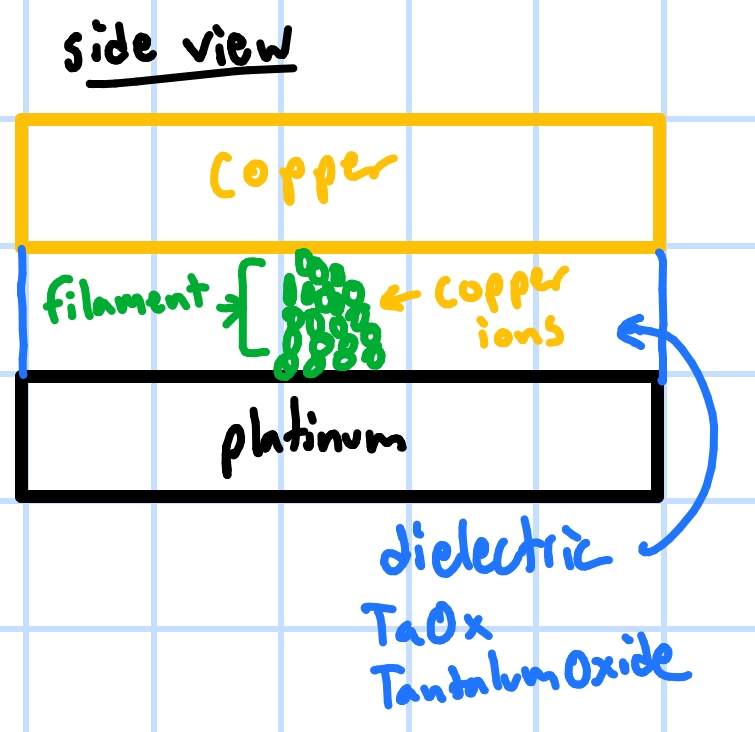
\includegraphics[width=10cm]{./figures/sideview_drawing.jpg}
            \caption{Simplified side view of a single memory cell}
            \label{sideview}
          \end{figure}
          \begin{figure}[H]
            \centering
            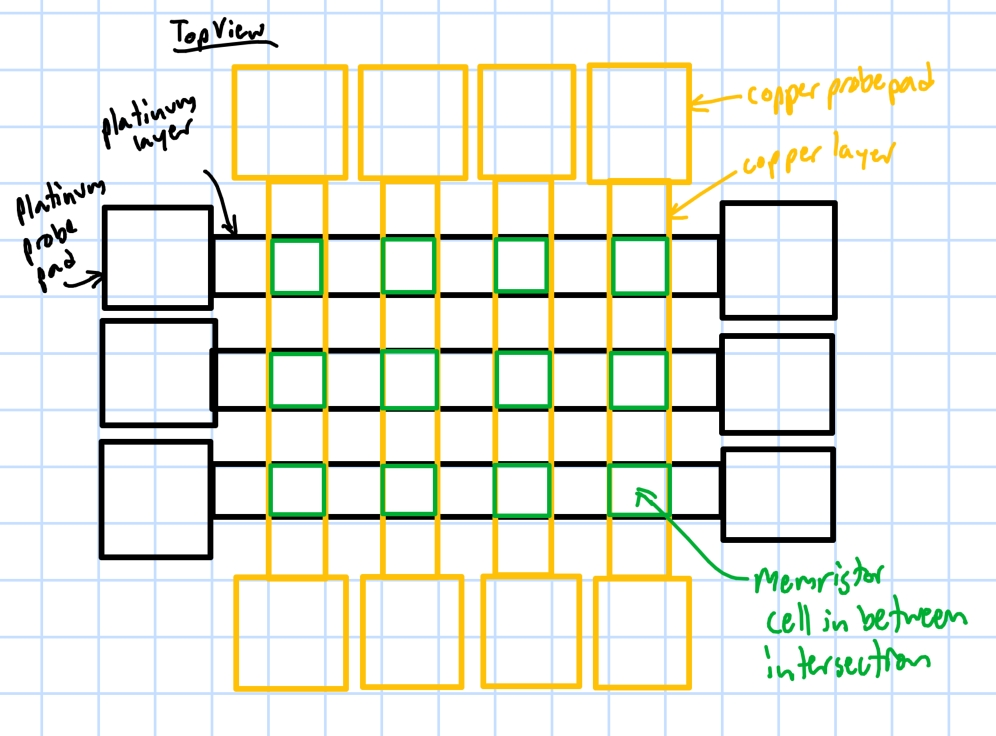
\includegraphics[width=\textwidth]{./figures/topview_drawing.jpg}
            \caption{Simplified top view of a single device array}
            \label{topview}
          \end{figure}

          Note that a Logic 0 or 1 is represented in the cell by virtue of the resistance measured across it.

          Note that a current limit (referred to as the \textbf{compliance current -- $I_{CC}$}) needs to be enforced to
          the supply of any voltages applied to the cell in order to avoid thermal runaway which would destroy the
          device entirely. $I_{CC}$ controls the thickness/strength of the filament. If $I_{CC}$ is too high, the
          filament will be too strong and we wont be able to reset the memory cell later (i.e.\ remove the filament).
          $5\mu A < I_{CC} < 70\mu A$ as given by Dr.Orlowski. In some cases we may use $I_{CC} > 70\mu A$ (e.g.\
          $260\mu A$) to demonstrate that a $cell_n$ that was set with a strong filament can be resilient towards the
          heat transfer from the switching of $cell_t$ (see Section~\ref{solution} for nomenclature and context
          references).

          In order to create the filament on a fresh device, a voltage $V_{form}$ is required to be applied between the
          layers. This will be done via a linear ramp from $0V$ to $V_{form}$, and will remain at $V_{form}$ until the
          compliance current is hit. Alternatively, a potential $> V_{form}$ can be applied in order for the compliance
          to be hit faster, below a certain limit (4.5-5$V$). This can be seen in the line labelled `(1)' in
          Figure~\ref{setCurve} below. Once this is done the memory cell is considered set.

          Then in order to set or reset the memory cell, the filament will have to be `built-up' or `weakened'
          respectively. This can be done by applying a potential $V_{set}$ or $V_{reset}$ accordingly. The length of
          time for which a potential has to applied can be determined by the current flowing through the device (which
          we will measure), as this is a direct indication of the state of the filament, and by extension the resistance
          of the filament. As can be seen in Figure~\ref{setCurve}, once $V_{reset}$ is hit, because the filament will
          have been weakened significantly, no current flows and the curve drops back to an $I$ of effectively 0A. The
          same logic as described in the previous paragraph with regards to potentials $> V_{form}$ applies to $V_{set}$
          and $V_{reset}$.

          \begin{figure}[H]
            \centering
            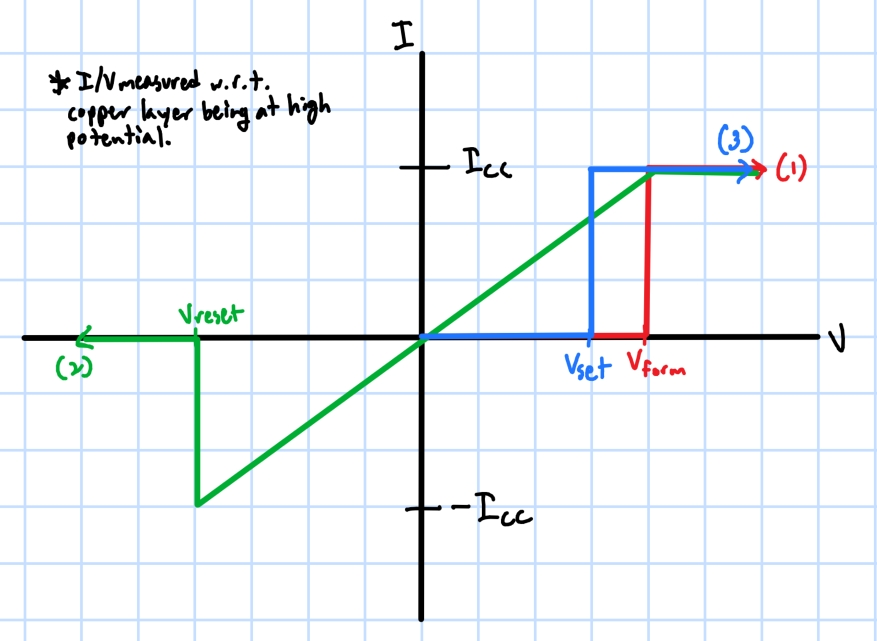
\includegraphics[width=10cm]{./figures/characterizationcurve.jpg}
            \caption{$I-V$ Curve showing $V_{form}$, $V_{set}$, and $V_{reset}$}
            \label{setCurve}
          \end{figure}

          The realistic construction of the ReRAM array devices we will be working on can be seen in the
          Figure~\ref{realview} below.
          \begin{figure}[H]
            \centering
            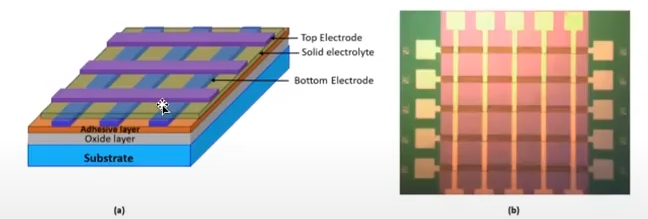
\includegraphics[width=\textwidth]{./figures/realview.jpg}
            \caption{Perspective of our device construction in reality}
            \label{realview}
          \end{figure}
        
        \newpage
        \subsubsection{Terminology} \label{terminology}
          \begin{itemize}
            \item [] \textbf{Filament:} The conductive path between the copper and platinum layers made up of copper
            ions.
            \item [] \textbf{Electrode:} Each `line' in the top or bottom layer of copper or platinum.
            \item [] \textbf{Cell:} The volume of the intersection between a copper and platinum electrode where the
            filament is formed. This is the memory cell that we check the resistance of in order to determine whether a
            logic 0 or 1 has been stored in it. The cell can also be referred to as a \textbf{Memristor}. Amrita will
            often refer to this as \textbf{device} as well. No matter the array type, the edge-to-edge distance between
            any neighboring cell will always be $150\mu$m -- this is a result of the design of the grid design we are
            using. 
            \item [] \textbf{Dielectric:} The material in between each electrode within which the cells form. In our lab
            is Tantalum Oxide (TaOx), and is only slightly opaque.
            \item [] \textbf{Contact Pad:} The which our probes contact in order to get continuity with the electrodes.
            \item [] \textbf{Array:} An arrangement of electrodes with platinum in columns and copper in rows, the
            intersections between which are where our filaments are formed. For the wafers we are handling, these are
            only 1 layer deep - i.e. the stackup is just copperElectrode--TaOx(FilamentLayer)--PlatinumElectrode, as
            opposed to
            copperElectrode--TaOx(FilamentLayer)--PlatinumElectrode--TaOx(FilamentLayer)--copperElectrode--...
            \item [] \textbf{Grid:} A matrix-ish arrangement of arrays on each wafer half. See coordinate system
            description and Figure~\ref{gridcoordinate} below for how arrays are mapped in each grid. The layout of the
            grid is determined by the mask we use, which is expensive and complicated to acquire, so we only use the one
            that Amrita and the lab have been using -- meaning that we will only ever deal with only type of Grid type.
            \item [] \textbf{Device:} The arrangement of material stackup for a grid -- Amrita and the lab personnel
            have multiple varieties. For our scope, these variances only occur in material thicknesses within our
            general Copper-TaOX-Platinum and substrate stackup. Each stackup, differed in terms of the thicknesses of
            each layer in said stack up, are referred to by `Device $x$' where $x$ is typically some 2 digit number. The
            final wafer that we will be using for data collection (see Section~\ref{solution}) will be 150nm copper,
            25nm TaOx, and 50nm Platinum -- referred to as Device \textit{<unassigned>}. Amrita has a pdf of a set of
            drawings labelling all the device variances. We will only be using device 43 and 44 -- 43 is characterized
            by having 100nm copper layer, whist 44 has a 130nm copper layer. This $x$ number is typically written in
            sharpie on the underside of the wafer. 
            \item [] \textbf{Wafer:} The silicon wafer upon which each half has a grid of the same device type. The
            wafers are then cut in half. These are grown by Amrita in the photolithography lab. We run our experiments
            on these. Amrita only has a single photolithography mask for growing our ReRAM grids on the wafers, so this
            is a major constraint. It usually takes her 14 straight hours to grow a set of grids from scratch on a
            single wafer, although she plans to make atleast 1 new one within the Spring 2021 semester so that we can
            observe cell formation using $V_{form}$. The other wafers are old in the order of years old, so and most of
            their cells have been formed already.
          \end{itemize}

        \newpage
        \subsubsection{Photolithography Process \& Wafer Coordinate System} \label{coordinatesystem}
        
          The Mask governs the pattern etched on the wafer. A fresh wafer is a circle with a small portion of its
          perimeter straightened, which is called the `primary flat'. Figure~\ref{mask} below is an image of the mask.
          Notice it has shapes grouped on 4 sides of the mask - we'll call these the North South East West Quadrants.
          During photolithography, only the northern quadrant is what is focused on, and is where the final arrays will
          end up when the process is done. Between each step in the photolithography process, the Mask is rotated
          $90^\circ$, then $180^\circ$, then $90^\circ$. If you look at Figure~\ref{mask} you can see each quadrant is
          slightly different, but their `macro' grid layout is the same. This is because each quadrant is responsible
          for etching different features of the arrays. Because our final arrays only coincide with the positioning of
          the northern quadrant, our wafer will only have a finished grid of arrays on one half of it. For convenience
          we cut the wafer in half, resulting in what can be seen in Figure~\ref{waferdone} -- this is the final wafer
          that we use in our experiments.

          In order to locate any cell in any array in any wafer of any device configuration reliably and consistently,
          we need to come up with a coordinate system and naming convention. Figure~\ref{gridcoordinate} is a screenshot
          of a portion of the mask with each of the arrays in our standard grid numbered. The pattern of this numbering
          should be self evident. Cells within arrays are then referenced in a 2dimensional coordinate system with the
          origin in the bottom left corner of the array. A clean standardized format for referencing a cell is as
          follows
          \begin{align} \label{namingconvention}
            \text{location}(\text{cell}_i) &= (d_0, r_0, c_0, r_1, c_1, r_2, c_2) \\
            \text{where } & d_0 \text{ is device type.} \notag \\
            \text{where } & r_0 \text{ is the primary row number (the red number in Figure~\ref{gridcoordinate})}\notag \\
            \text{where } & c_0 \text{ is the primary column number (the green number in Figure~\ref{gridcoordinate})}\notag \\
            \text{where } & r_1 \text{ is the secondary row number (the blue number in Figure~\ref{gridcoordinate})}\notag \\
            \text{where } & c_1 \text{ is the secondary column number (the yellow number in Figure~\ref{gridcoordinate})}\notag \\
            \text{where } & r_2 \text{ is the row of the cell in the array defined by $(d_0, r_0, c_0, r_1, c_1)$}\notag \\
            \text{where } & c_2 \text{ is the column of the cell in the array defined by $(d_0, r_0, c_0, r_1, c_1)$}\notag
          \end{align}

          If any detail from eqn~\ref{namingconvention} does not to be articulated or is not applicable for whatever
          reason, then place a `-1' in where necessary. For example, Figure~\ref{grid_3} is photo of the probes
          measuring a certain cell in a certain array. Correlating this photo to our grid layout shown in
          Figure~\ref{gridcoordinate}, we can surmise that the wafer is upside down and we are looking at the cell
          identified by $(-1, 4, 7, -1, -1, 0, 4)$. $d_0$ is -1 because I forgot to record what the the device type was
          in this image. $r_1, c_1$ are -1 because these parameters are irrelevant for this particular array (observe
          Figure~\ref{gridcoordinate} to see which ones they are relevant for). If for whatever reason we were not able
          to use contextual clues to zero in on the position of the array in the grid, $r_0, c_0$ would have both been
          -1 too.

          \begin{figure}[H]
            \centering
            \includegraphics[width=\textwidth]{figures/mask.jpg}
            \caption{The mask we use with all 4 quadrants in view.}
            \label{mask}
          \end{figure}
          \begin{figure}[H]
            \centering
            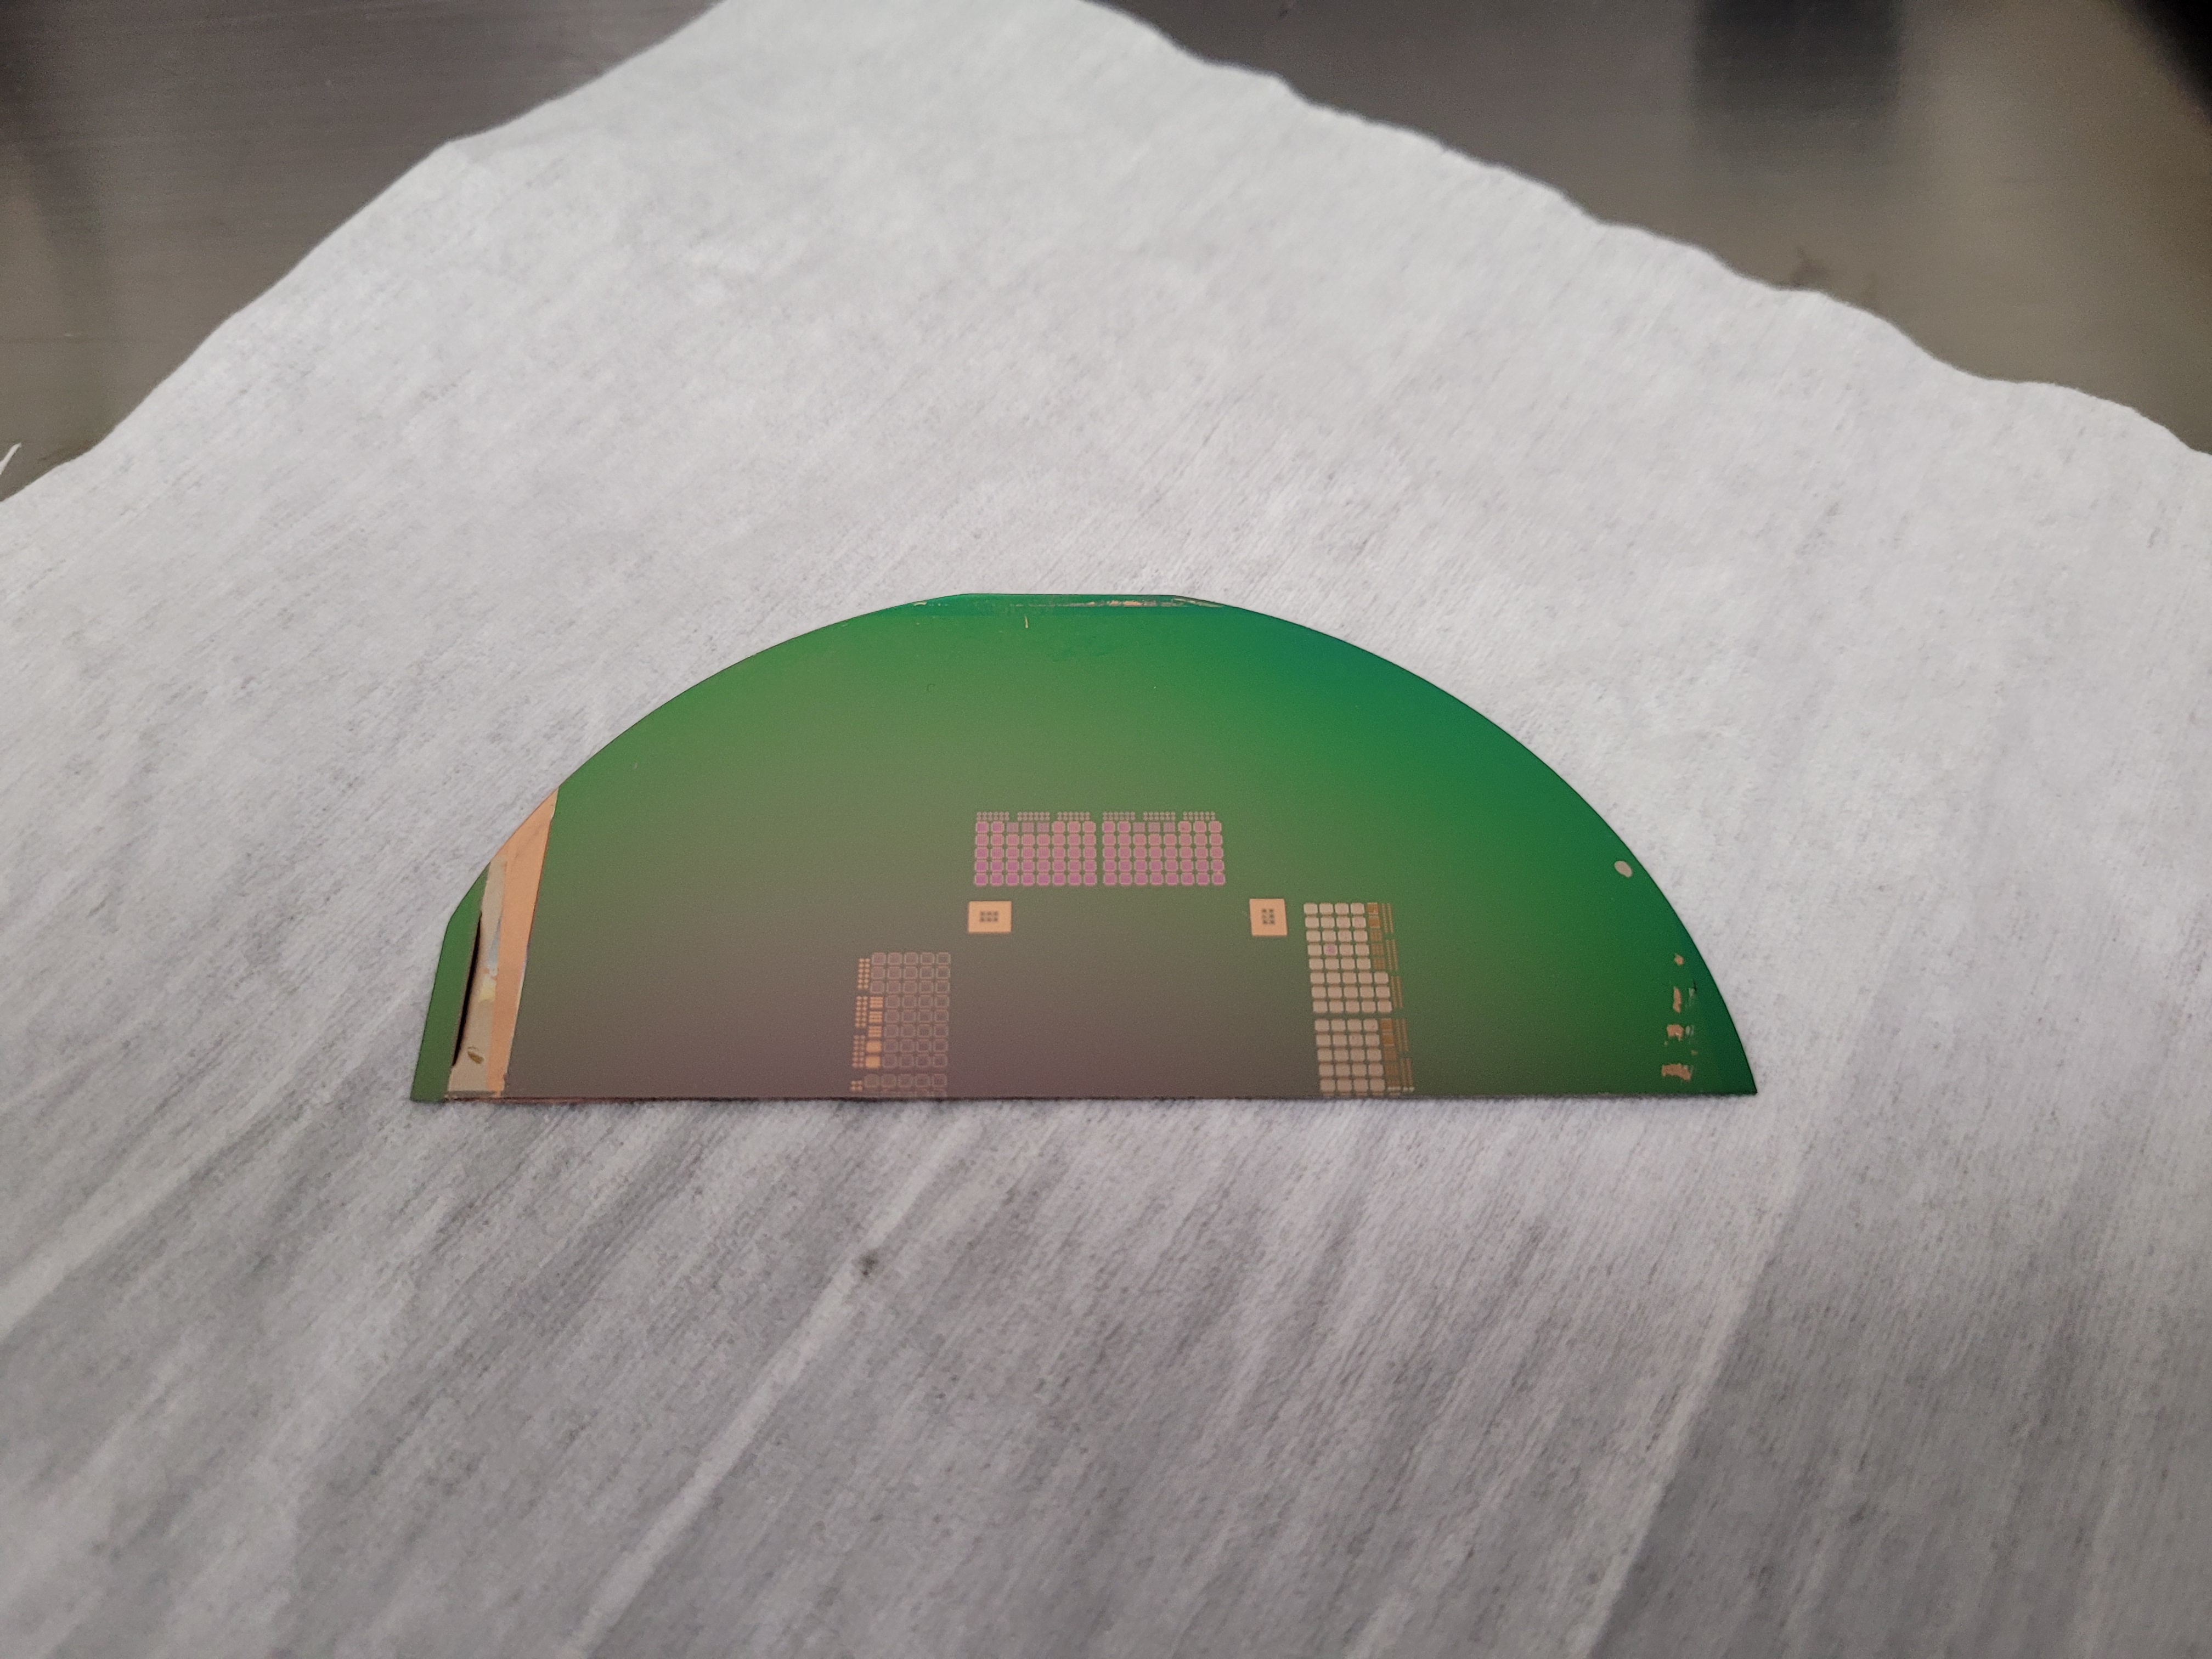
\includegraphics[width=\textwidth]{figures/waferdone.jpg}
            \caption{A finished and cut wafer that we use all the time. Notice the flats on the top and side of the
            wafer. These are irrelevant. Also notice the grids that appear on the sides that seem cutoff. These are
            artifacts of the mask and its 4 quadrants during the etch-rotate photolithography process we described
            earlier -- they are incomplete. The complete arrays that we use are located in the grid at the top.}
            \label{waferdone}
          \end{figure}
          \begin{figure}[H]
            \centering
            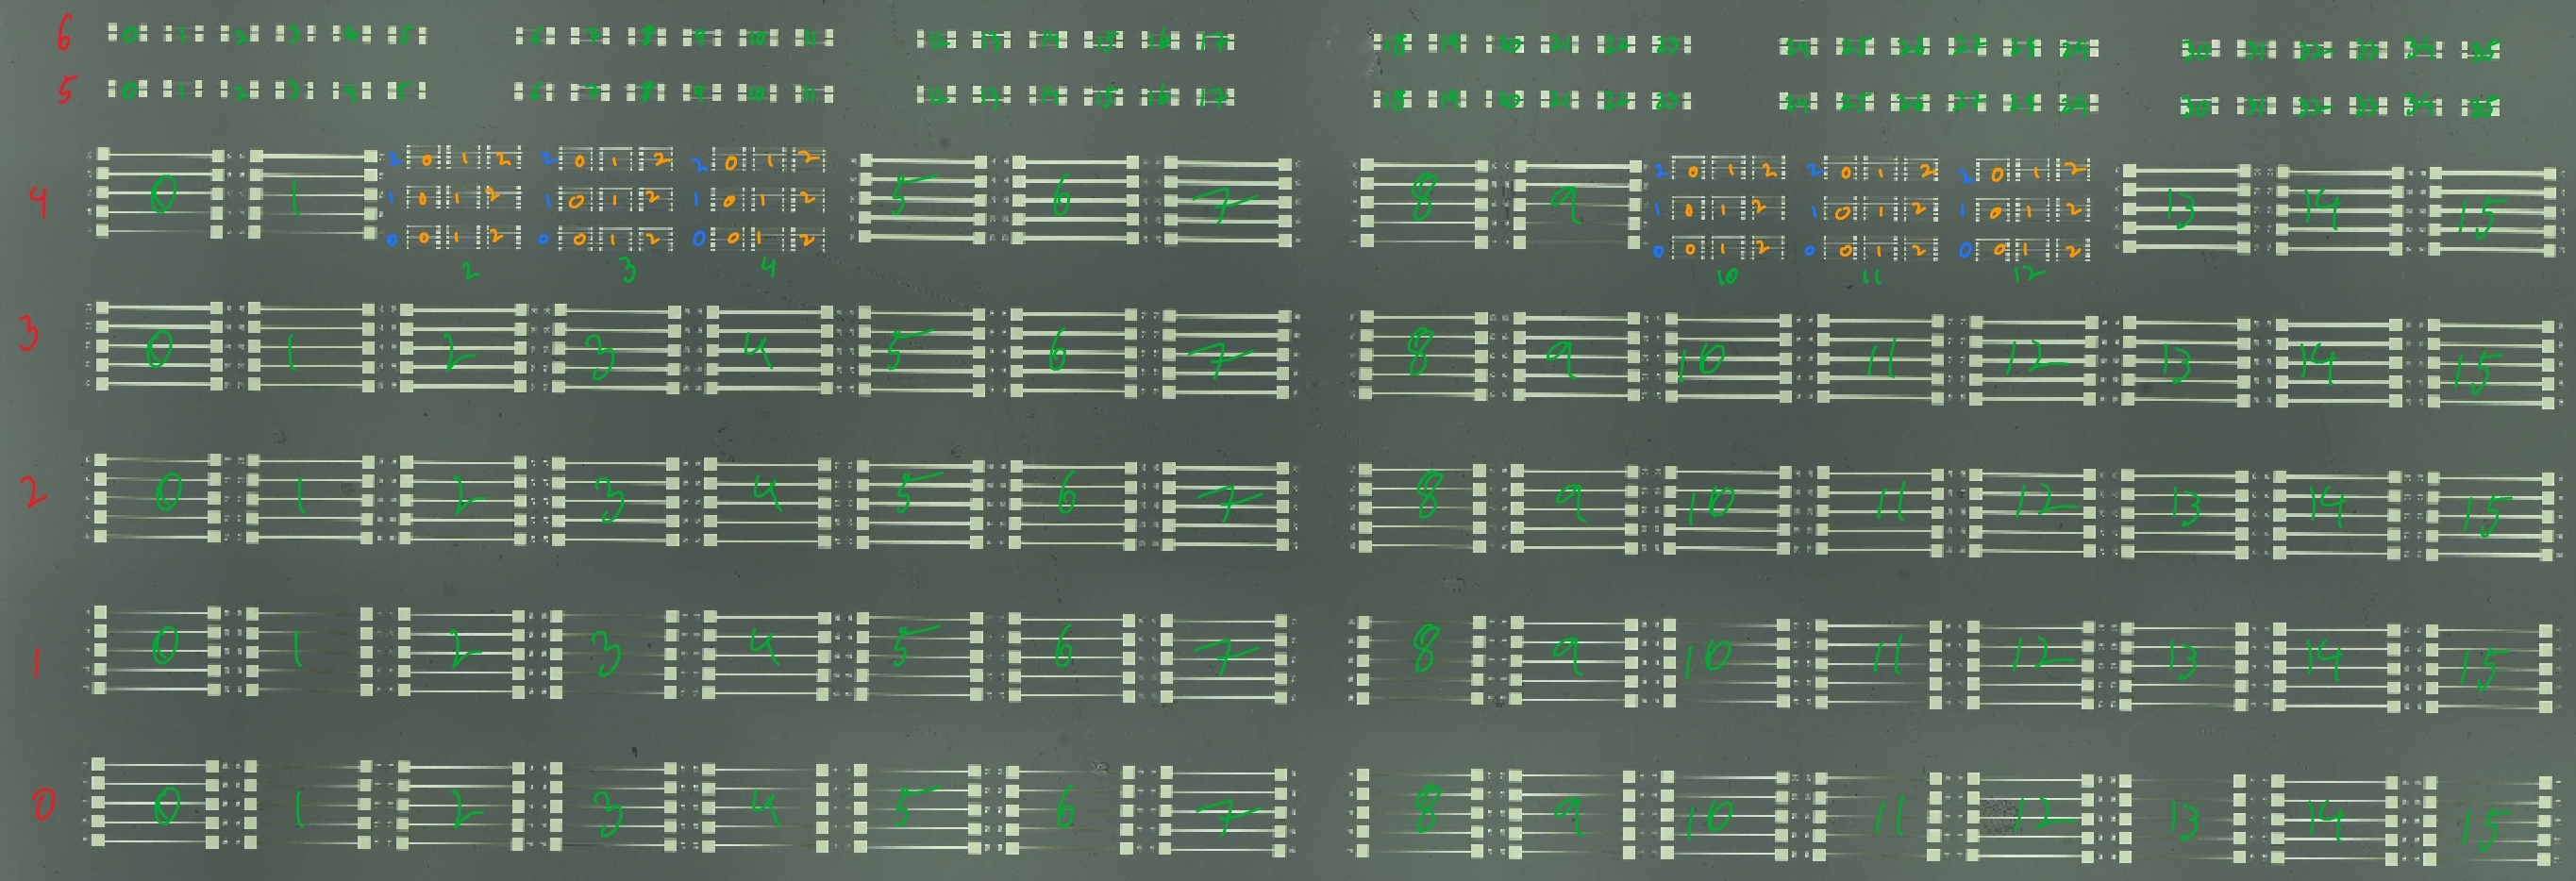
\includegraphics[width=\textwidth]{figures/maskcoord.jpg}
            \caption{An illustration of the grid coordinate system.}
            \label{gridcoordinate}
          \end{figure}
          \begin{figure}[H]
            \centering
            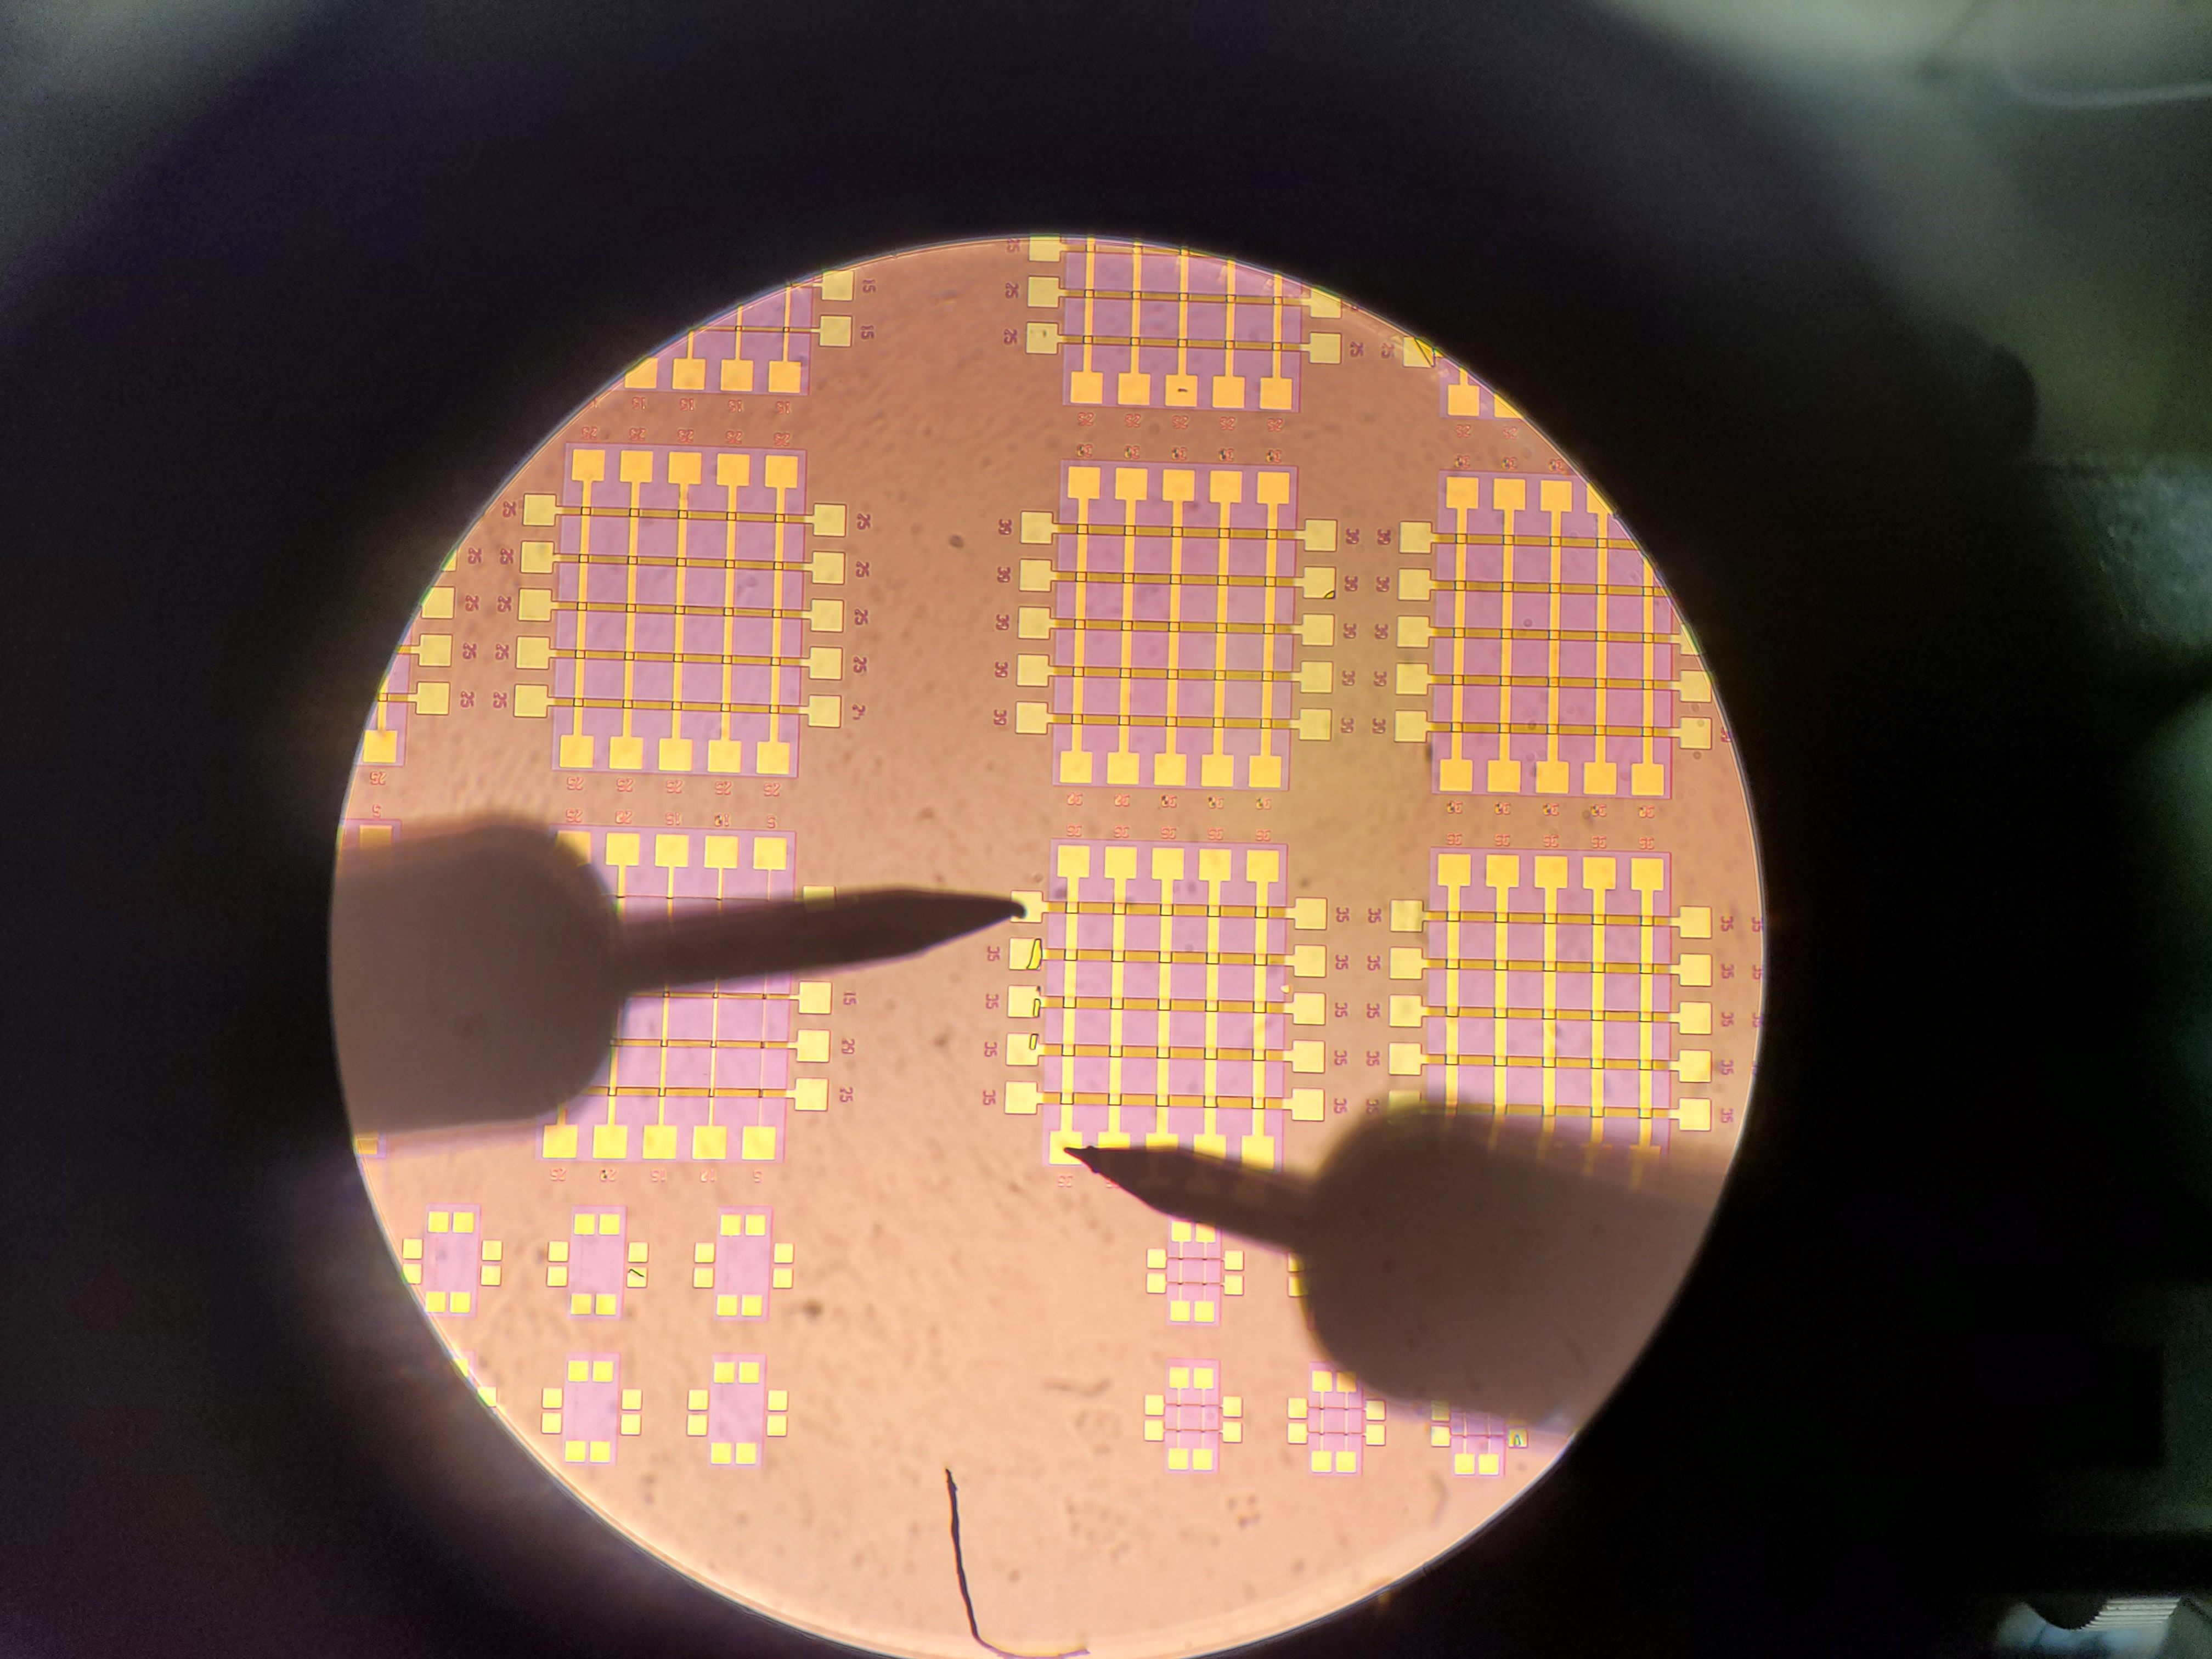
\includegraphics[width=\textwidth]{figures/microscope_grid_3.jpg}
            \caption{A photo of the microscope view of us targeting the cell at $(-1, 4, 7, -1, -1, 0, 4)$. The pinkish
              square encapsulating the cells in the arrays is the TaOx dielectric -- the middle layer. Below it is the
              platinum layer, the electrode contact pads for which are located just outside the pinkish square. At the
              top is the copper layer, the electrode contact pads for which look as if they are contained within the
              pinkish square.}
            \label{grid_3}
          \end{figure}

        \newpage
        \subsubsection{(TODO) Thermal effects on electron tunneling in neighbors}
            
          \textit{Explain how two levels of thermal energy in a filament (from switching within a period of time) result
            in copper ion displacements, as well as filament conduction degradation, as explained in video in our shared
            google drive -- https://drive.google.com/file/d/1HNudbTjQwhGMvVA0n-Gc4JBXrSSjBQt3/view?usp=sharing.}    
      
      \newpage
      \subsection{Who are we working with}
        Dr. Orlowski is the lab director and in charge of the Micron Lab at Virginia Tech, overseeing the Micron
        research work as a whole. Dr. Orlowski is as our SME, and potentially will have to play the role of customer as
        well.

        Amrita Chakraborty is one of our Senior Design GTA's, as well as the main point of contact for all
        clean-room/semiconductor related senior design projects. We work with her very closely, and she is the one that
        guides lab familiarization and day to day hands-on project work. Amrita assumes the role of SME as well.

        Zuzanna is our contact with Micron, however communication has been lackluster -- no reply on the first outreach,
        followed by a reply after an email reminder, followed by no reply once again. She would potentially be our
        customer, or would have put us in touch with other Micron employees who would be better suited, or even just for
        more exposure. But with the non-determinism of communication, to assign her as customer seems risky. 
        
        As of the 2022 Spring semester our customer is no longer a representative at Micron – this was established after
        an entire semester’s worth of effort in keeping up correspondence with Micron proving indirectly that they were
        not interested in the role-playing aspect of this senior design project. Amrita Chakraborty will act as our SME
        and Dr.\ Orlowski as our customer – this assignment is far more appropriate and closer to the reality of how our
        project has been panning out: Amrita helps us facilitate lab equipment and procedures as well as being a direct
        source of expertise in the knowledge-area of our project; Dr.\ Orlowski is the director of the Micron research
        efforts at Virginia Tech among which Amrita’s PhD research efforts is a part, our project is guided in the ‘big
        picture’ by biweekly meetings with Dr.\ Orlowski, and we are in consistent communication with Amrita throughout
        the week.
      
      \newpage
      \subsection{What are we being asked to do} 
        The ultimate aim of this project is for us to investigate the effects a target cell's neighbor's states as a
        result of setting and resetting said target cell. From empirical experience in the past, Dr. Orlowski and his
        lab have observed strange quantum behavior on the states of neighboring cells whereby their states were changed
        from their resting states, and non-deterministically returned to their original resting states an unknown amount
        of time later. These effects are said to be occurring due to the thermal changes in the device around the target
        cell as a result of the setting/resetting of the target cell.

        Our job would be to figure out a reliable and repeatable way in which to manipulate the device and collect data
        that illustrates the behavior mentioned above. However doing this is challenging as their are many lab and
        equipment dependent constraints in play, described in Section~\ref{resources and constraints}.
        Section~\ref{solution} details our final solution. 

        % \subsubsection{Timeline of Goals} \label{goaltimeline} \begin{itemize} % [$\boxtimes$] to checkmark \item
        % [$\boxtimes$] Complete all lab training and equipment familiarity by \textbf{October 2021}. \item [$\square$]
        % Practice and achieve proficiency in characterizing memory cells as described in Figure~\ref{setCurve} by
        % \textbf{December 2021}. This and the previous step anticipated to take up all if not most of the Fall semester
        % (i.e.\ the first half of our 1-year timeline). All practice on old wafers with oxidation damage. \item
        % [$\square$] Amrita completes new fresh wafer for us to collect main data on, by \textbf{November 2021}. Until
        % then practice set reset cycles (where possible) on old wafers, as well as 3 probe setup and honing in on
        % automation scripts. \item [$\square$] By end of \textbf{January 2021} start forming target cells (e.g. center
        % and corners for each array) and neighbor cells in a variety of array types within the new wafer's grid. Setup
        % database, and get automation software in working order. \item [$\square$] By end of \textbf{February 2021}
        % finish collecting all data. Start preparing final statistical analysis' of data, as well as documentation on
        % navigating database. Also get started with final posters/presentations preparations. \item [$\square$] For
        % each device stack up (defined in Section~\ref{day2day}) find the respective $V_{form}$, $V_{set}$ and
        % $V_{reset}$ independently and without Amrita's input. Get conclusions based on tests on multiple cells on
        % multiple grids. Submit our results to Amrita so she can correlate our findings with their own and confirm both
        % our accuracy and the lab's knowledge. by \textbf{month\_? 2021}. Depending on pace of progression we may only
        % stick to one device stackup. \item [$\square$] Formulate experimental plan to collect neighbor cell data and
        % manipulate target cell given all constraints by \textbf{month\_? 2021}. \item [$\square$] Collect data
        % according to formulated experimental plan between by \textbf{month\_? 2021} and by \textbf{month\_? 2021}.
        % \item [$\square$] Process and summarize findings by \textbf{month\_? 2021}. Some data analytics and general
        % data cleanup would be nice. Unknown if expected to analyze data and reach conclusions due to lack of expertise
        % in device science and quantum physics. \end{itemize}
        
      \newpage
      \subsection{The resources we have and their constraints} \label{resources and constraints}

        \subsubsection{Lab} \label{lab} 
        
          We will be working in Whittemore 617, which contains all the lab equipment. Figure~\ref{wholeapparatus} is a
          wide shot of our entire setup, with the probe-microscope bench, and the Keithley machine in view.

          \begin{figure}[H]
            \centering
            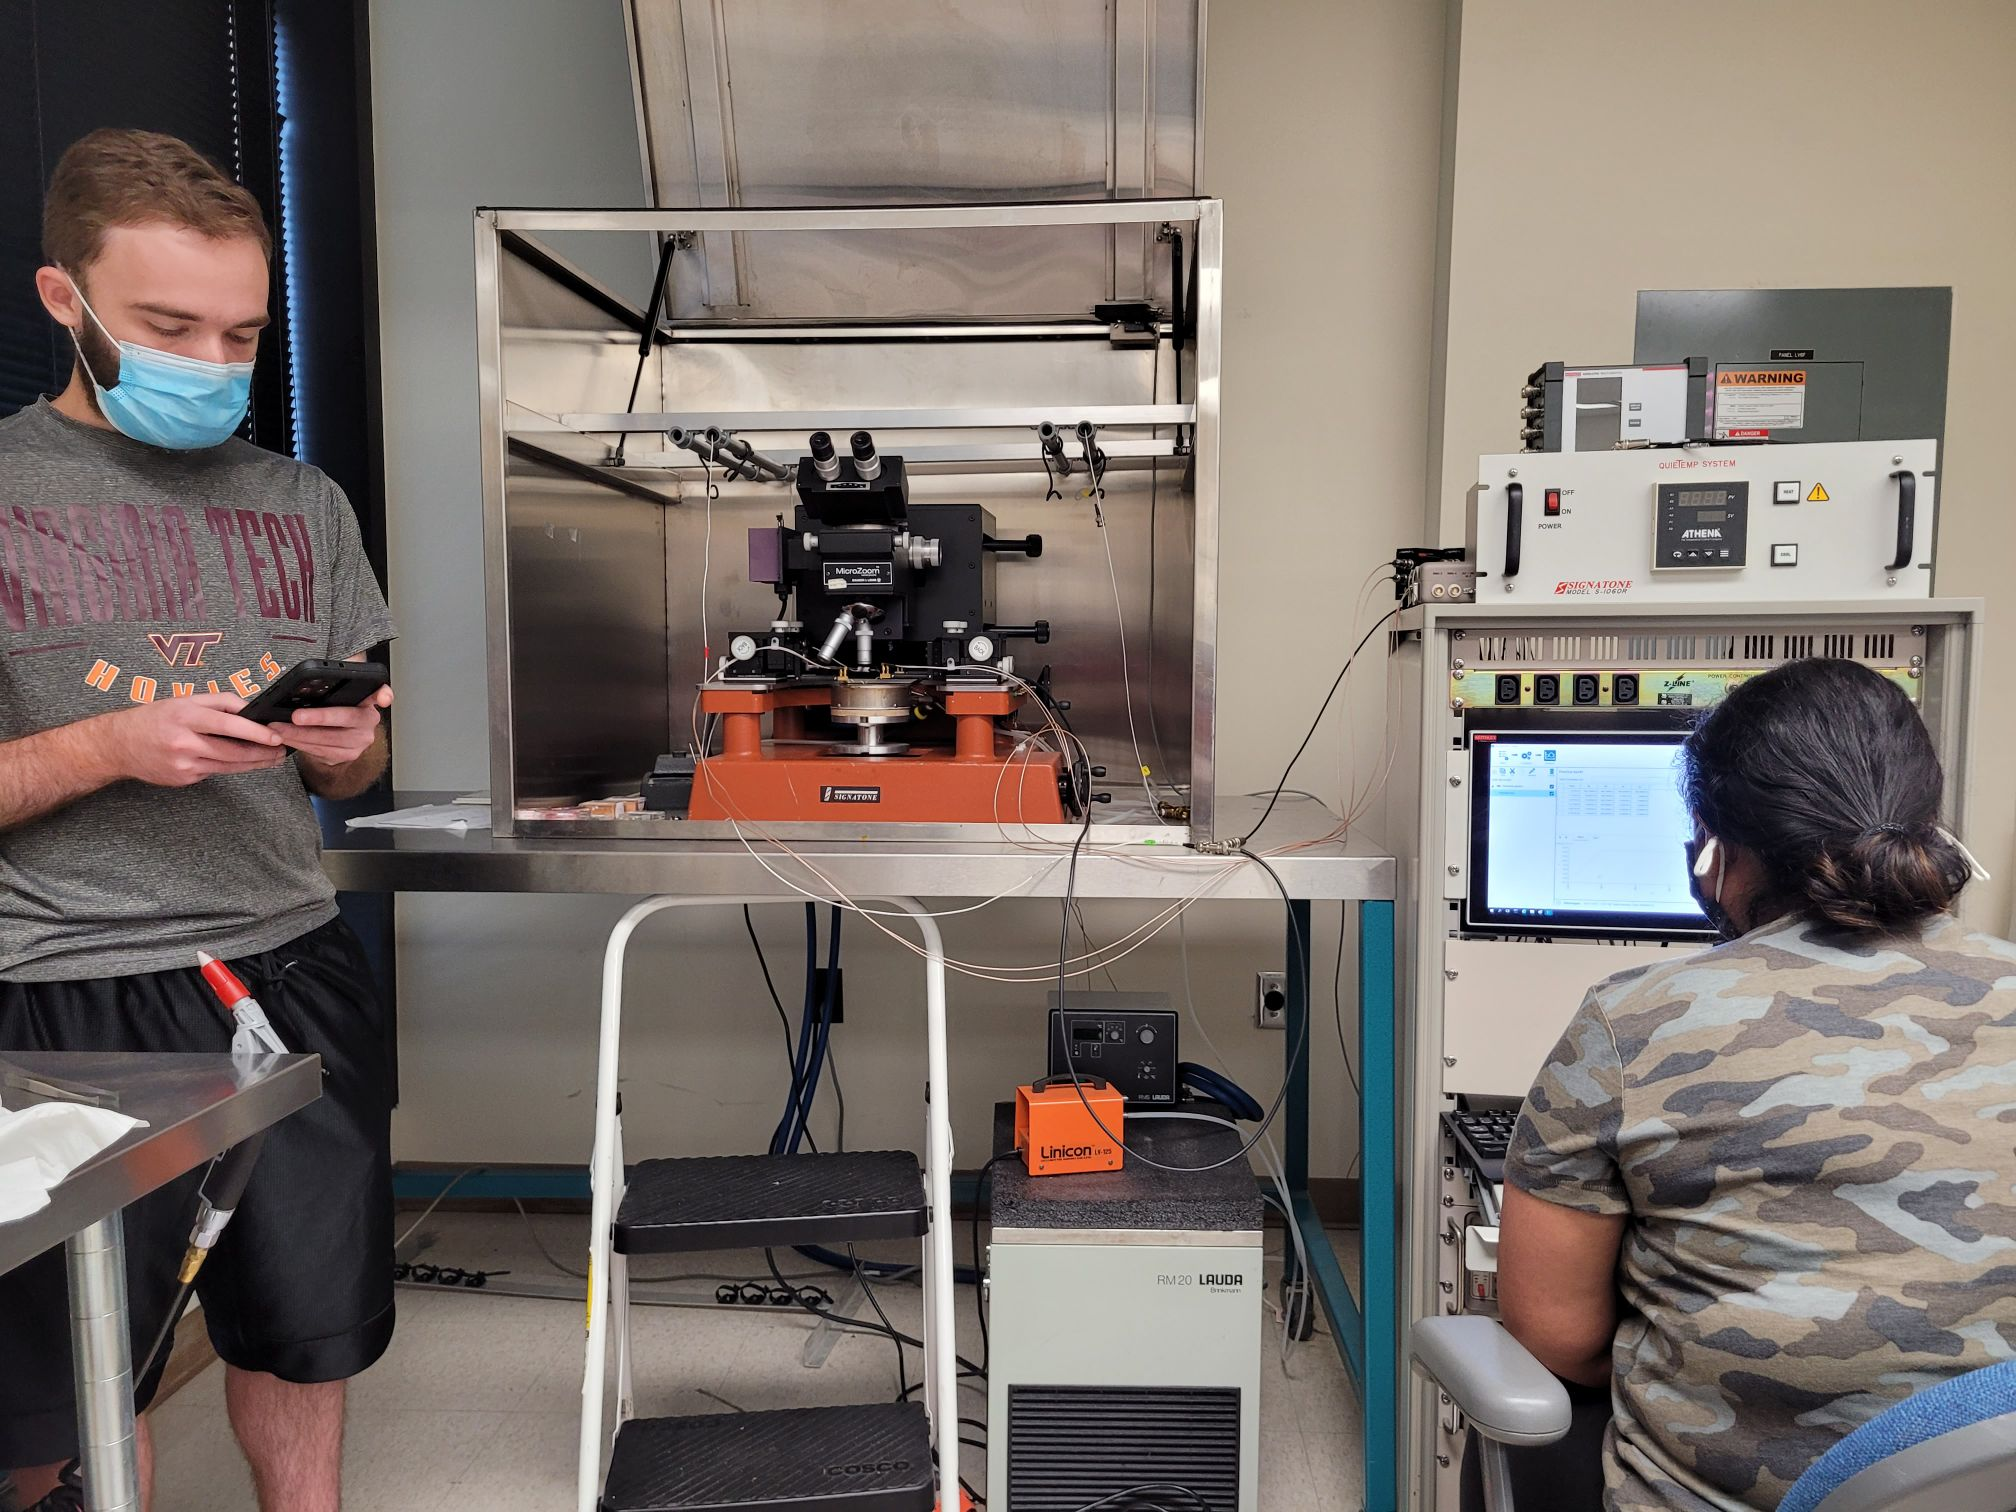
\includegraphics[width=10cm]{figures/apparatuswhole.jpg}
            \caption{Nick, Amrita, the Probe-Microscope bench, and the Keithley Machine, all in one lovely picture.}
            \label{wholeapparatus}
          \end{figure}

          \underline{List of Contraints}
          \begin{itemize}
            \item Access during weekdays during working hours.
            \item Amrita needs to be present.
          \end{itemize}
        
        \newpage
        \subsubsection{Keithley Machine - Keithley 4200A-SCS} 
          Figure~\ref{keithley} shows what the Keithley Machine looks like. The interface is pretty much like a
          computer. It even runs windows 10. The purpose of the machine is to act as a precision power supply,
          measurement device, and data logger for our micro electronics experiments. Currently, the software we use
          within the Keithley machine to do all of this is called Clarius, the GUI of which can be seen in
          Figure~\ref{clarius2}.

          \begin{figure}[H]
            \centering
            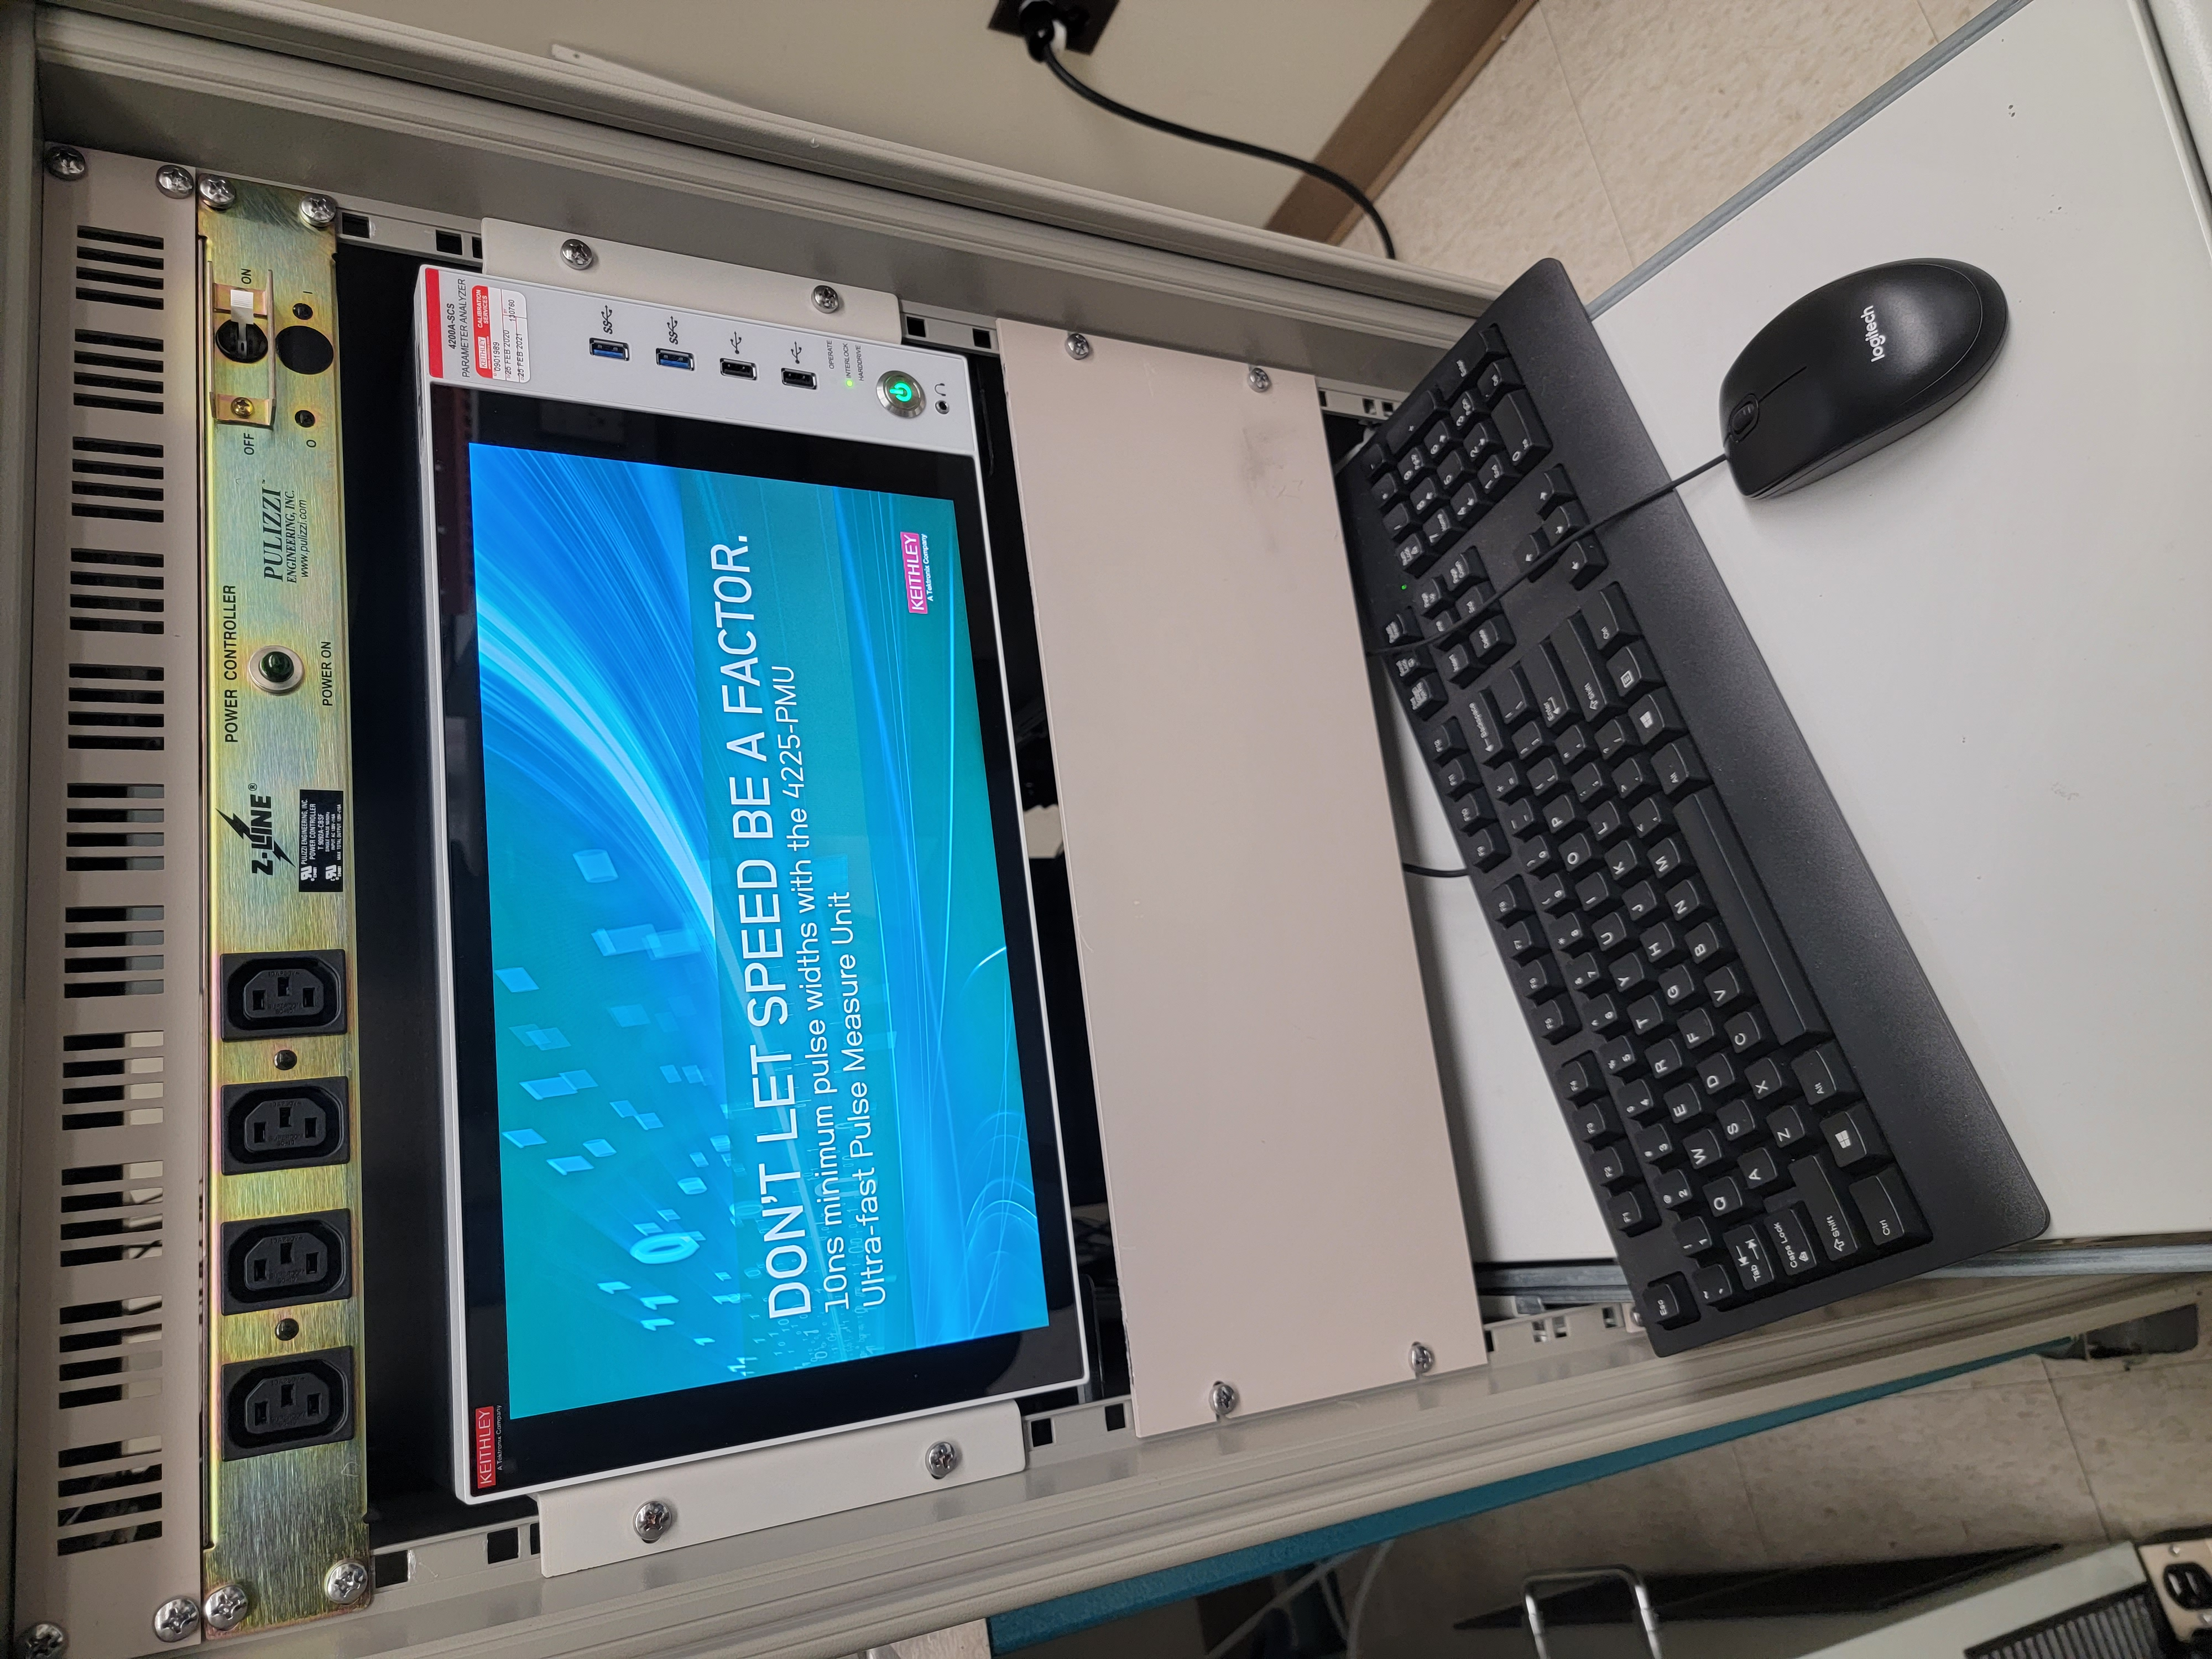
\includegraphics[width=10cm]{figures/KeithleyMachine.jpg}
            \caption{The Keithley machine. Idk why \LaTeX\; insists on making this image sideways.}
            \label{keithley}
          \end{figure}
          \begin{figure}[H]
            \centering
            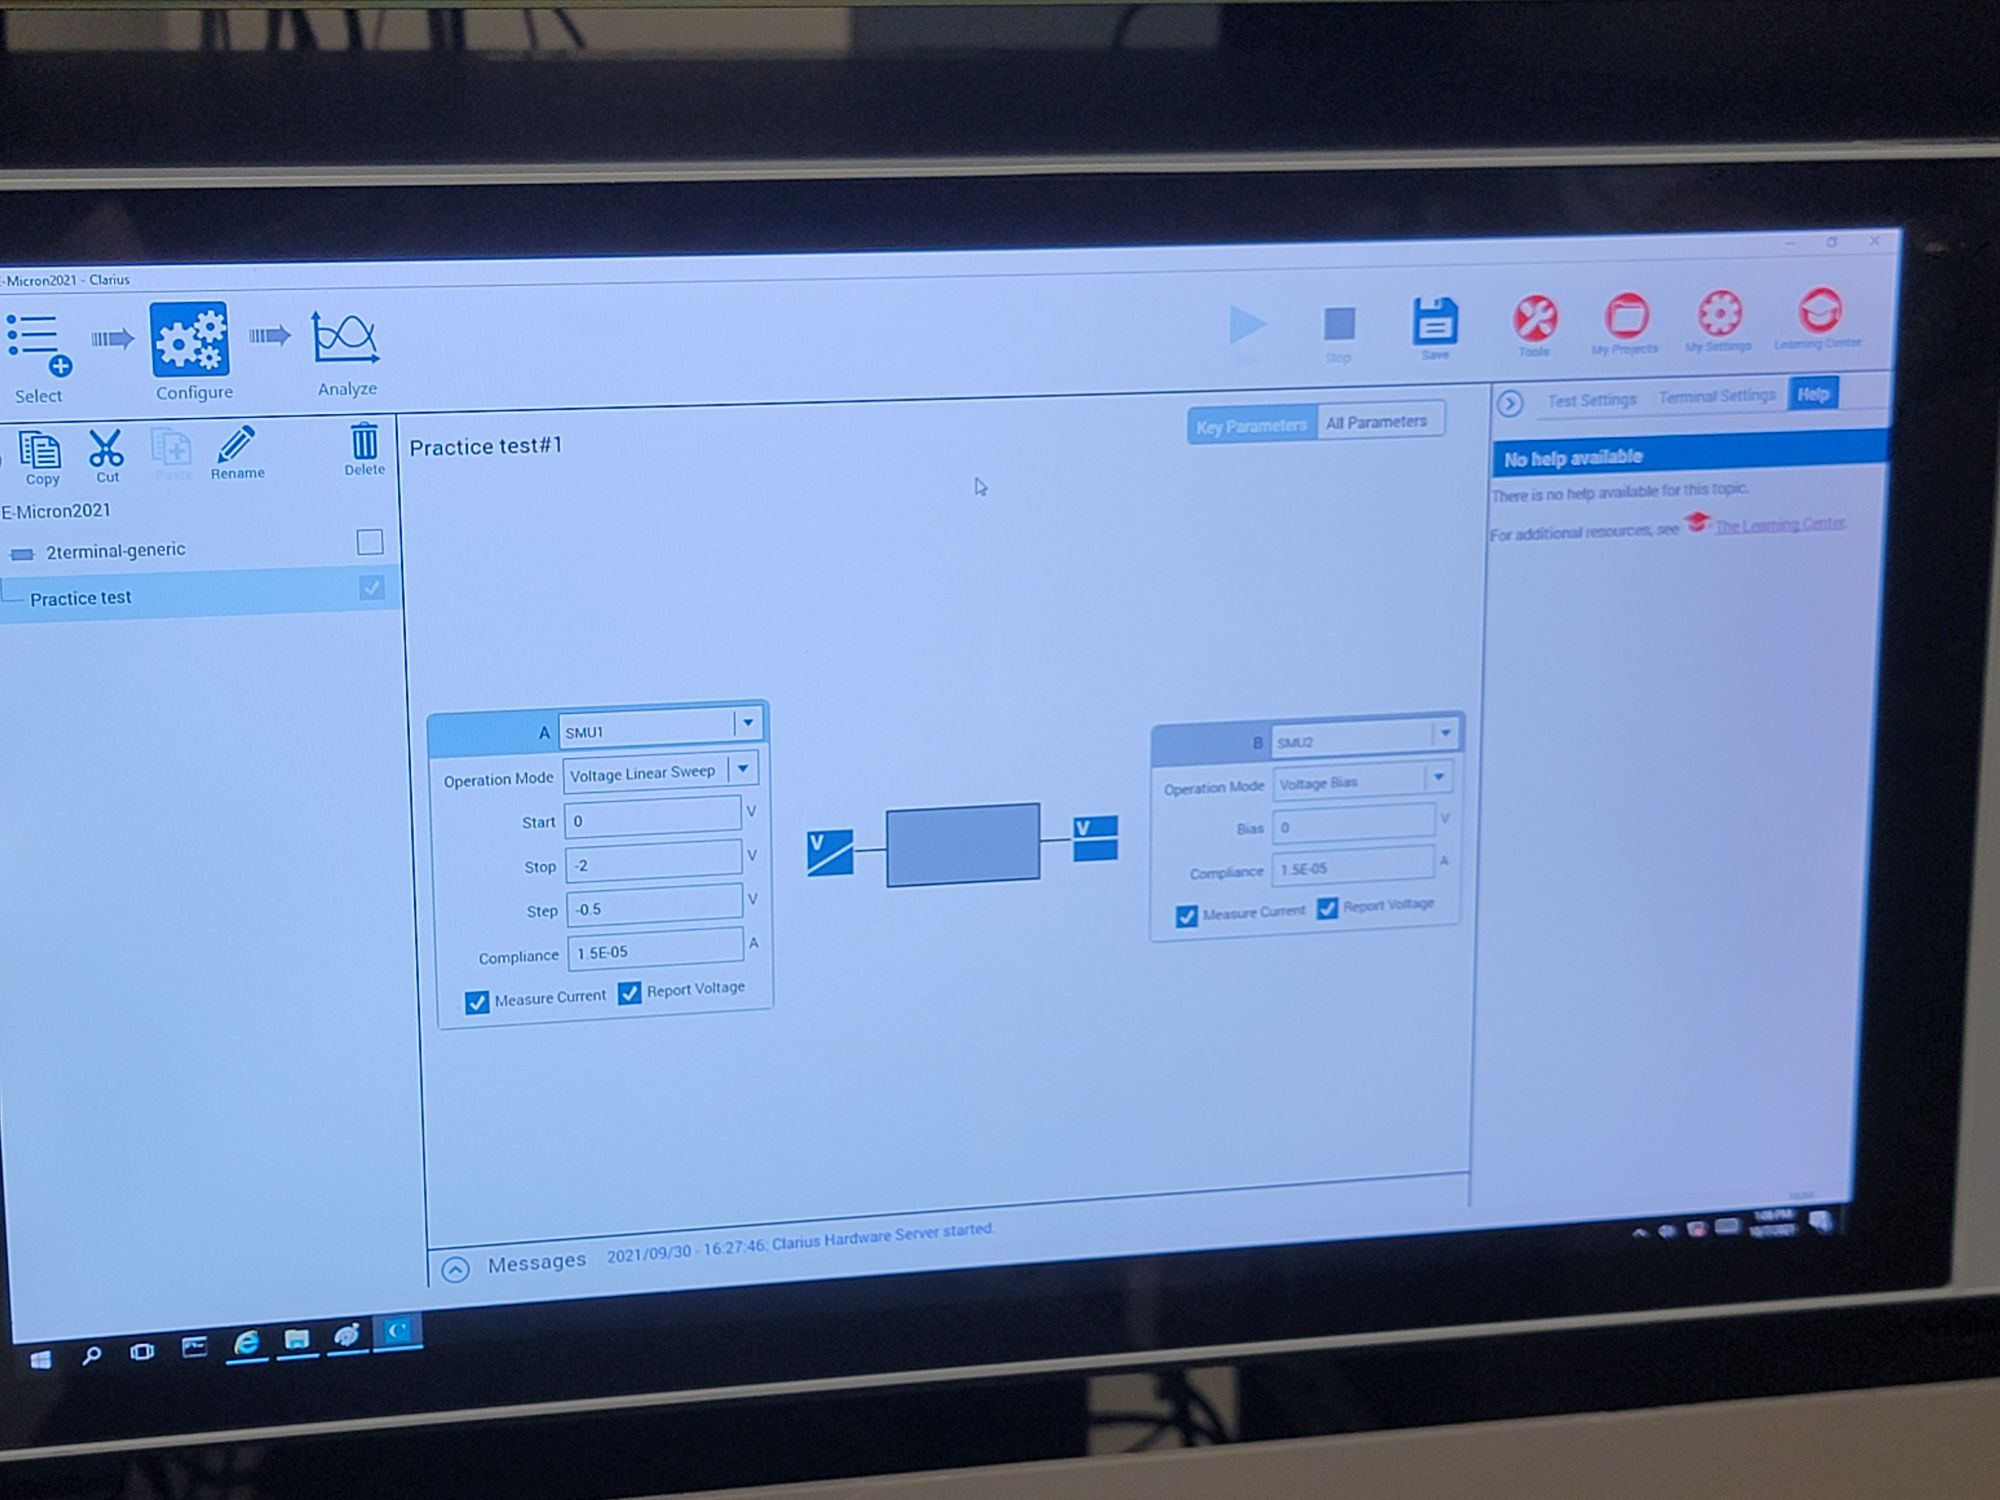
\includegraphics[width=10cm]{figures/clarius_2.jpg}
            \caption{What the clarius software on the keithley machine looks like.}
            \label{clarius2}
          \end{figure}

          \underline{List of Contraints}
          \begin{itemize}
            \item list constraints here \textit{(note from Dr.\ Orlowski: the team may brainstorm the constraints
            perceived during the project so far. It would be a great legacy for the future teams working on this
            technology and be aware of some possible showstoppers.)}
          \end{itemize}
        
        \newpage
        \subsubsection{Probe-Microscope Setup}
          Figure~\ref{probemicro} shows our probe microscope setup. The black things with the knobs are what the probes
          are attached to. They allow for precise movement of the probes in space.

          \textit{TODO!: talk about probes, the 4 wire setup and reasoning, its limitations etc.}
          
          \begin{figure}[H]
            \centering
            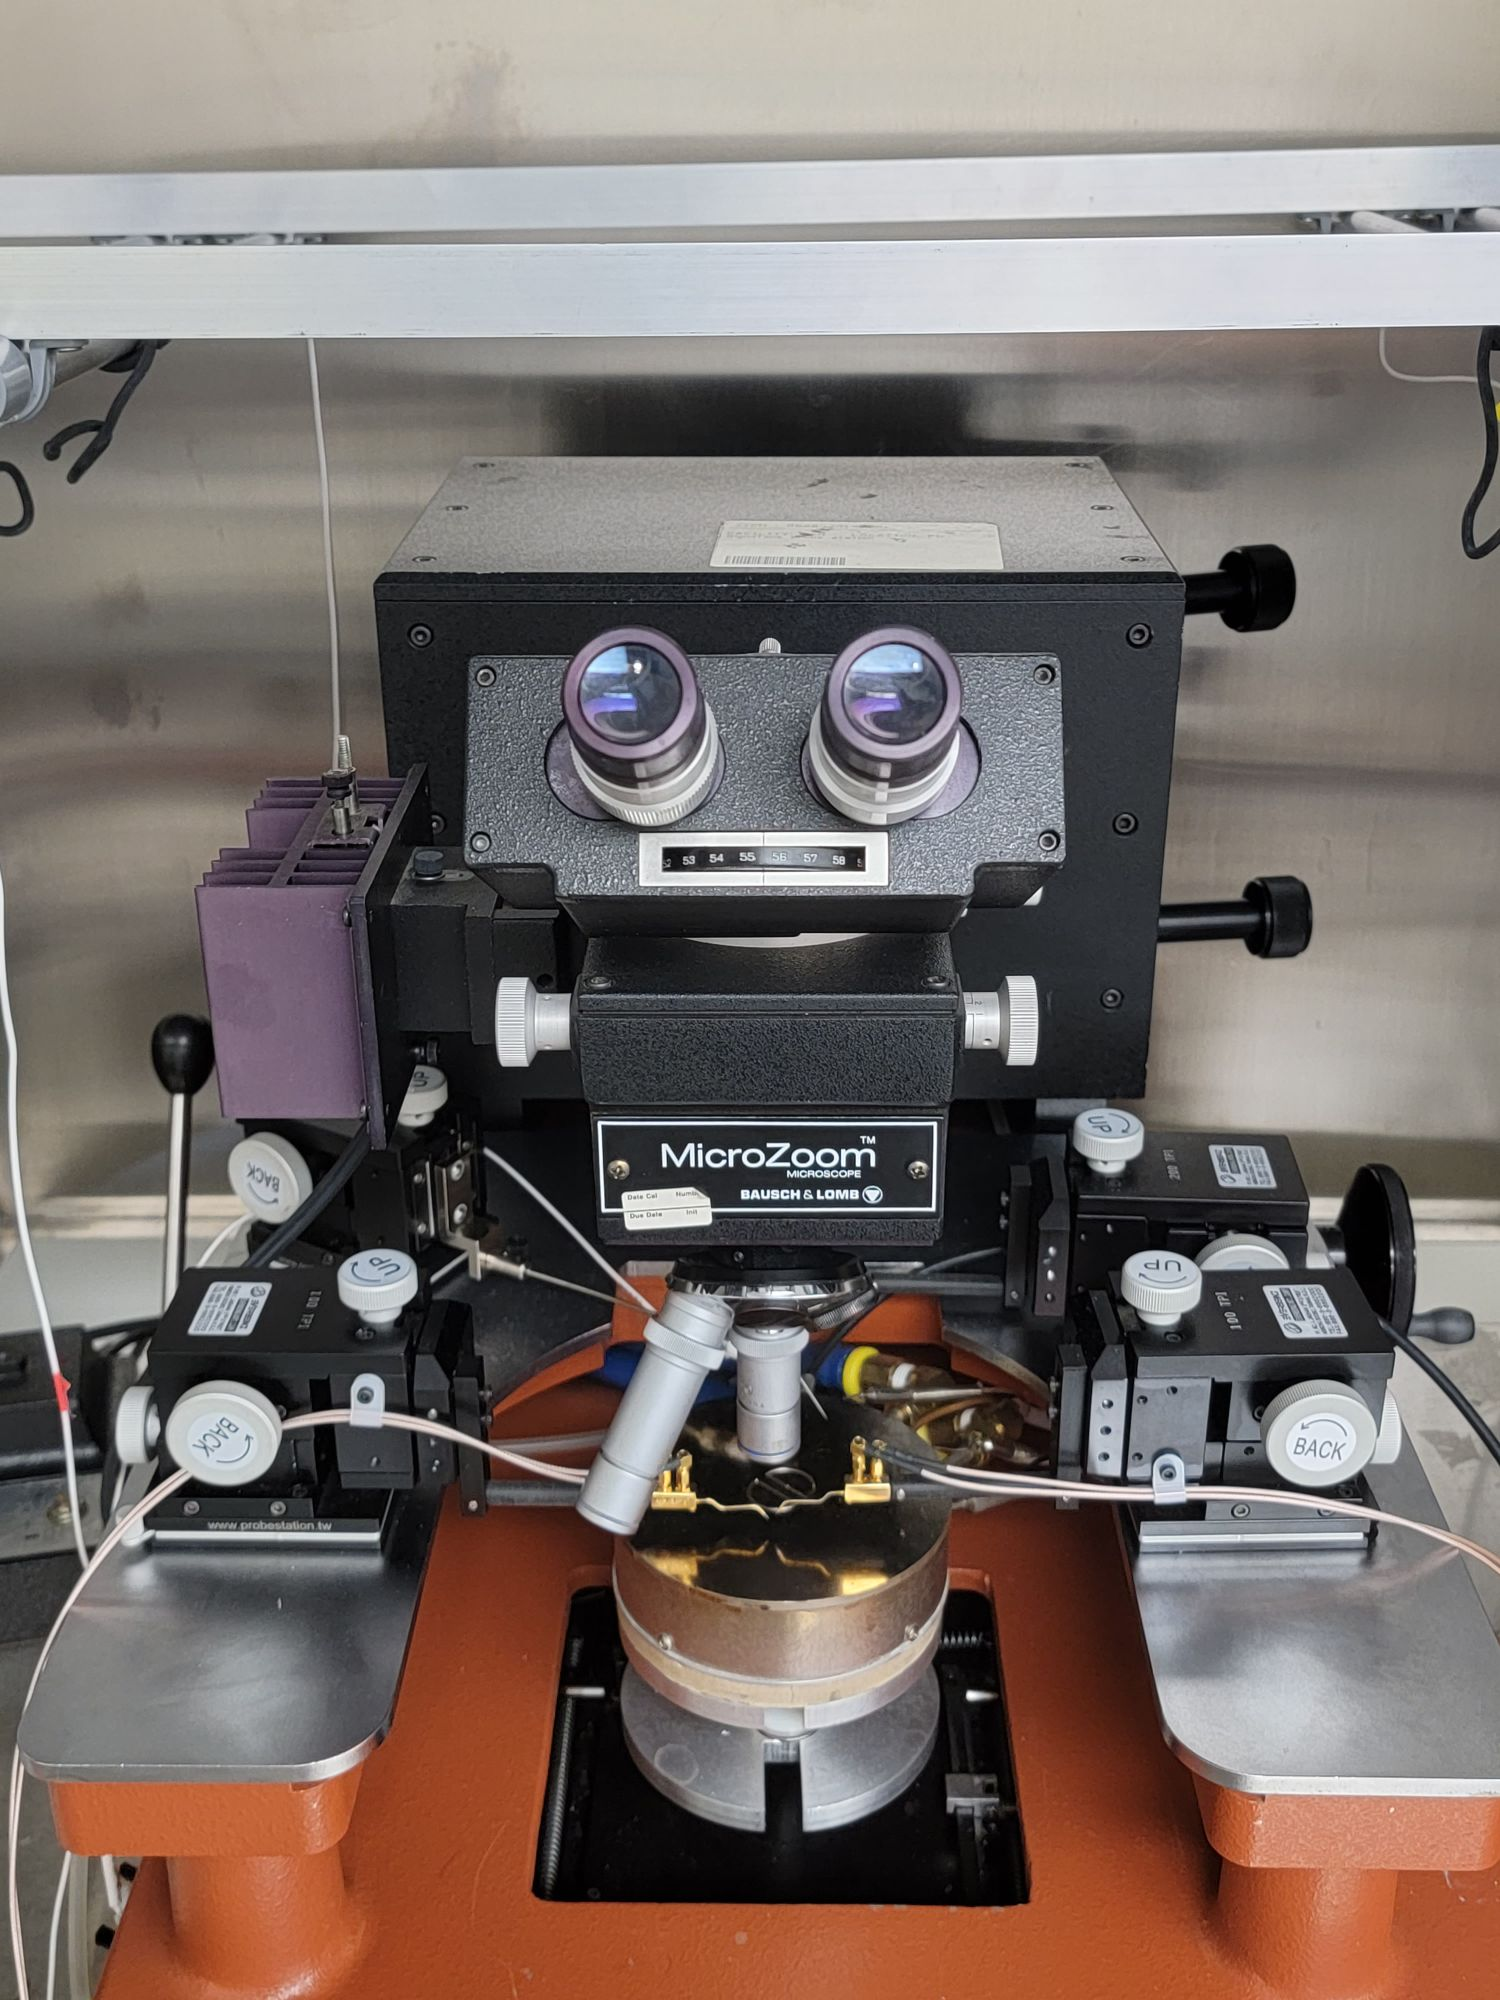
\includegraphics[width=10cm]{figures/probeapparatus_front.jpg}
            \caption{A front-on view of the probe-microscope setup.}
            \label{probemicro}
          \end{figure}

          \underline{List of Contraints}
          \begin{itemize}
            \item 4 probes in setup. No choice about this thats how its setup. Currently (and for the foreseeable
            future) only 3 probes exist. Meaning we can only contact 3 contact pads. The implications of this is that
            the neighbors we can observe must be perpendicular to our target cell as they would share a common ground.
            To observe a diagonal neighbor would require a separate reference ground and therefore 2 extra probes beyond
            the 2 used for manipulation of the target cell.
          \end{itemize}

        \newpage
        \subsubsection{PMU's} 
          \textit{enter description here -- general description, its interfaces, software, etc}

          \underline{List of Contraints}
          \begin{itemize}
            \item list constraints here.
          \end{itemize}
        
        \newpage
        \subsubsection{Grid on Wafer Setup} 
          \textit{enter description here -- general description, its interfaces, software, etc}

          \underline{List of Contraints}
          \begin{itemize}
            \item New wafers with new sets of grids on them takes Amrita 14 straight hours to make. Most of the ones on
            hand are already pretty old. She estimates to make at least one new one in the Spring 2021 semester for us
            to be able to observe cell setting using $V_{form}$. We will mostly be using old wafers on the order of
            years old, the cells of which have been set a long time ago.
            \item Mask is fixed and pre fabricated. A new one cannot be made. So the arrangements and sizing of grids on
            the wafer is fixed to what we have. When doing bulk data collection we will need to cleverly work around the
            inefficiencies that arise from the way the grids are arranged in order to not be inhibitively slow.
          \end{itemize}
        
        \newpage
        \subsubsection{Consumables} \label{consumables} 
        
          Figure~\ref{tweezer} is a picture of the tweezer we use, which is very expensive (in the hundreds of dollars)
          due to its material properties that make it safe for handling raw wafers.

          \begin{figure}[H]
            \centering
            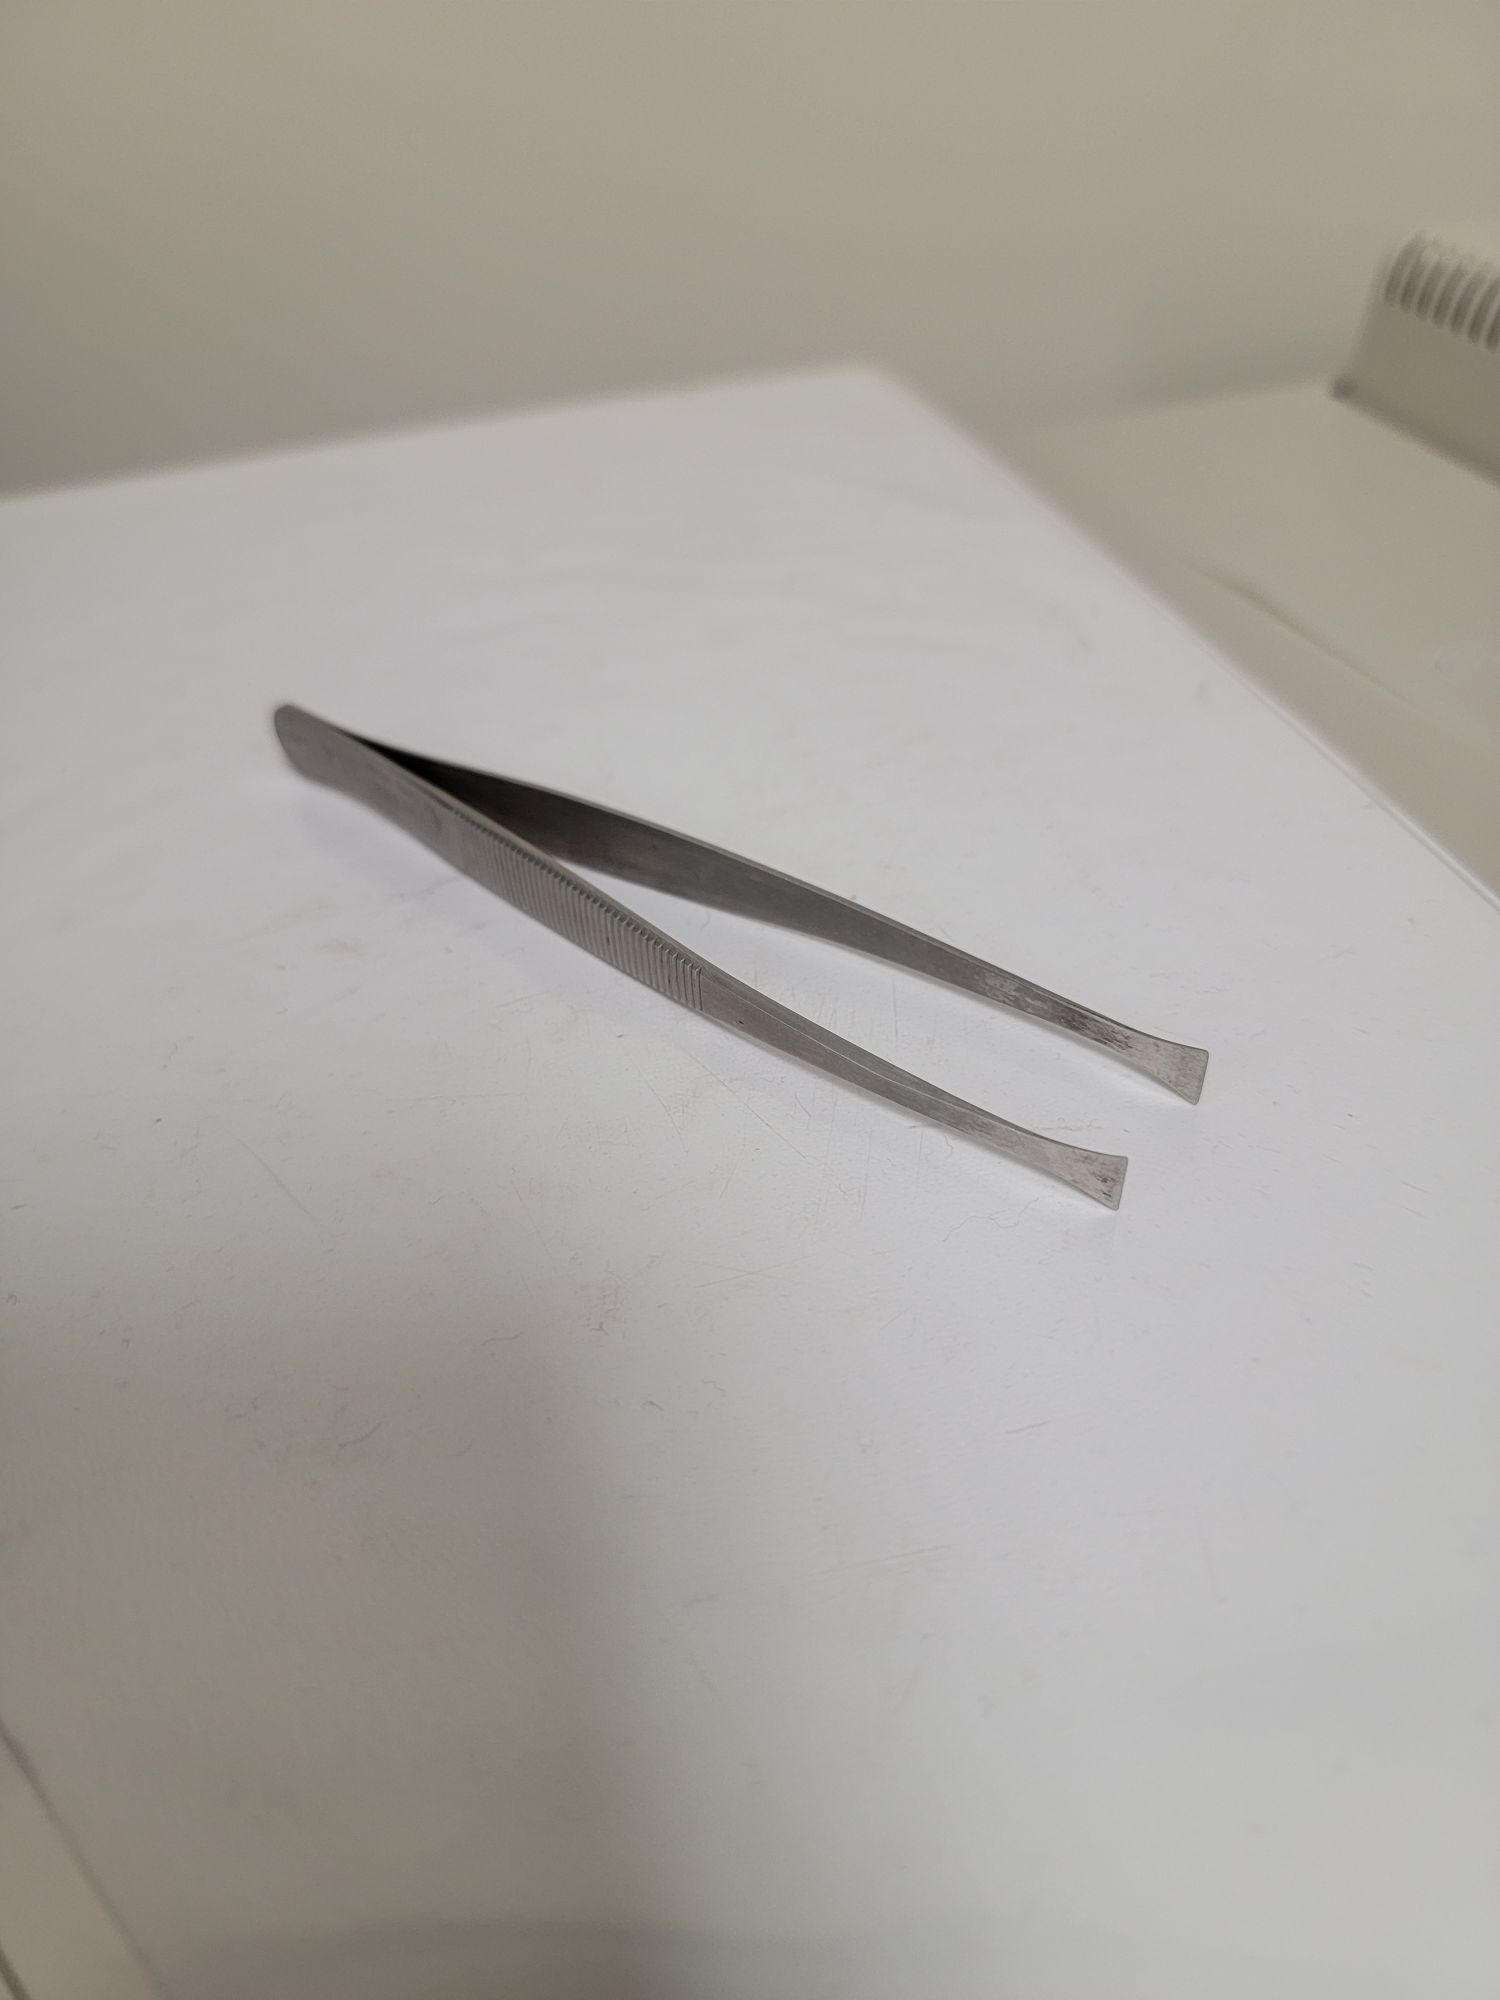
\includegraphics[width=10cm]{figures/tweezers.jpg}
            \caption{Our glorious and supreme tweezer. May it have mercy on us.}
            \label{tweezer}
          \end{figure}

          \underline{List of Contraints}
          \begin{itemize}
            \item 
          \end{itemize}  

    \section{Overall Solution Breakdown} \label{solution}
    
      \subsection{Data Collection Related Nomenclature} \label{nomenclature}

        Refer to section~\ref{terminology} for a reminder of what any certain ancillary term may mean.

        \begin{enumerate}
          \item [\textbf{$cell_t$} :] the target cell who's current and voltage we are manipulating.
          \item [\textbf{$cell_n$} :] the cell neighboring $cell_t$ who's voltage we fix and current we observe.
          \item [\textbf{Cell Pair} :] a single pair of $(cell_t, cell_n)$ that we manipulate and observe at any given
            point during our data collection.
          \item [\textbf{Cell Pair Set} :] the set of all cell pairs that we would like to manipulate and collect data
            for throughout the duration of our senior design project. Cell pairs can be varied in terms of what array
            type they lie in in the overall grid, as well as where in a particular array they could be situated. These
            positional factors can influence how thermal energy is transferred from $cell_t$ to $cell_n$, and by
            extension can also influence potentially differing behaviors we might notice in the set/reset status of
            $cell_n$ over time.
          \item [\textbf{$P_t$} :] the probe connected to $cell_t$.
          \item [\textbf{$P_n$} :] the probe connected to $cell_n$.
          \item [\textbf{$P_{gnd}$} :] the probe connected to the common ground between $cell_t$ and $cell_n$.
          \item [\textbf{$V_{P_t}$} :] The voltage that is applied to $cell_t$ through $P_t$. This will vary as a
            function of time during data collection. It is an independent variable/controlled input in our data
            collection.
          \item [\textbf{$Icc_{P_t}$} :] The compliance current (i.e.\ current limit) that is applied to $cell_t$
            through $P_t$. This will also vary as a function of time during data collection. It is an independent
            variable/controlled input in our data collection.
          \item[\textbf{$I_{P_t}$} :] The actual current that flows through $cell_t$ at any given point in time. This is
            a dependent variable/observed output in our data collection. 
          \item [\textbf{$V_{P_n}$} :] The voltage that is applied to $cell_n$ through $P_n$. This will stay constant
            throughout the data collection process as the purpose of $cell_n$ is just to observe whether or not it is
            set (by observing the current passing through it), which will be affected by the thermal energy produced
            from switching $cell_t$. It is an independent variable/controlled input in our data collection.
          \item [\textbf{$Icc_{P_n}$} :] The compliance current that is applied to $cell_n$ through $P_n$. This will
            stay constant throughout the data collection process for the same reason as above. It will be far less than
            $Icc_{P_t}$ because we only need to observe the set/reset condition of the filament in $cell_n$. It is an
            independent variable/controlled input in our data collection.
          \item[\textbf{$I_{P_n}$} :] The actual current that flows through $cell_n$ at any given point in time, which
            will tell us if a filament is formed or not in $cell_n$. This is a dependent variable/observed output in our
            data collection.
          \item[\textbf{$V_{P_t}$ shape} :] The arrangement of $V_{P_t}$ values against time that we would like the
            Keithley machine, programmed through clarius, to achieve when manipulating $cell_t$ according to our desired
            waveform.
          \item[\textbf{$Icc_{P_t}$ shape} :] The arrangement of $Icc_{P_t}$ values against time that we would like the
            Keithley machine, programmed through clarius, to achieve when manipulating $cell_t$ according to our desired
            waveform.
          \item[Run File :] In any clarius project we can create `run files', which when clicked on shows an arrangement
            of interconnected blocks that allow the user to select certain parameters with which to manipulate our $P_t,
            P_n,$ and $P_{gnd}$ probes. Then, when the play button at the top right of the GUI is hit, the probes are
            then influenced to output the parameters we described in the software. The Voltages of these probes can be
            arbitrarily manipulated against time in each Run File. However for each Run File, each probe can only have a
            single $Icc$ compliance current which cannot be manipulated. If a different $Icc$ is required, another
            subsequent Run File will be needed. Each run file will be named in the order in which it is executed, so the
            first run file with be '1', next will be '2' and so on.
          \item[Run Folder :] Each clarius project can contain multiple Run Files ordered under a single drop down. This
            drop down will be referred to as a Run Folder. If we click on a run folder and then hit `play' at the top
            right of the clarius GUI, then all the Run Files contained within it will be run in order. By cleverly
            arranging a series of Run Files we can achieve complete arbitrary control of $Icc$ and $V$ for any of our
            probes against time, as we desire. This will be essential in achieving our desired `test cycle', which will
            be described below.
          \item[Test Cyle :] A single test cycle is achieved by a specific ordered set of appropriately designed Run
            Files under a single Run Folder. When said Run Folder is 'played', a test cycle will be executed. An ideal
            test cycle can be defined by plotting certain $V$ and $Icc$ values against time for each probe. This ideal
            test cycle would describe how, in an ideal world, we would want to manipulate the parameters of our probes
            in order to achieve adequate stimulus of $cell_t$ in order to observe thermal-cycling effects in $cell_n$. 
            
            We can vary the set and reset $V$ shapes and $Icc$ shapes in our test cycle, as well as vary how often and
            with what frequency these various set and reset shapes will appear over time in our test cycle.
      
            Once this ideal test cycle is well defined, we would then work on replicating it as closely as possible by
            creating a series of Run Files within a single Run Folder.
        \end{enumerate}

      \subsection{Wafers Currently on Hand} \label{wafers}

        Details about wafers we have produced for the express purpose of data collection are referred below:

          \begin{itemize}
            \item [Wafer 1] 
              \begin{itemize}
                \item [] \textbf{Date Created :} ???
                \item [] \textbf{Comments :} Copper electrodes faulty. 23nm of Tantalum Oxide (manufacturing limit is
                  25nm). Platinum is 50nm and Copper is 150nm. Strange form and set behavior. Super short cell lifespan
                  of less than 5 to 10 cycles. 
              \end{itemize}
            \item [Wafer 2] 
              \begin{itemize}
                \item [] \textbf{Date Created :} 11th March 2022
                \item [] \textbf{Comments :} No faulty copper electrodes. 25nm of Tantalum Oxide. Platinum is 50nm and    
                  Copper is 150nm.
              \end{itemize}
          \end{itemize}

      
      \subsection{The Human Algorithm for Data Collection} \label{humanalgorithm}

        The following series of steps is run for each cell-pair in a pre-determined cell-pair set. This cell-pair set,
        and the positional and size variances within it, needs to be established before commencing data collection.
        
        \textit{The following steps have been deprecated. The same overall approach is still being used, however we are
        less hard-ass-ey about the details, as long as the ultimate goal (stated below) is achieved efficiently.}
        \begin{enumerate}
          \item \sout{Form and set $cell_n$ for every cell pair. With a fresh untouched wafer each $cell_n$ would have
            never been formed before.}
          \item \sout{Create a master directory called ``data''. Then, starting from the first cell-pair in the
            cell-pair set, do the following:}
          \begin{enumerate}
            \item \sout{Set $P_t$, $P_n$, and $P_{gnd}$ appropriately on the wafer according to the identified
              coordinates of the target cell-pair.}
            \item \sout{Click run the Run Folder representing the intended test cycle.}
            \item \sout{Collect the csv's produced by clarius into a thumb-drive, and name them with the following
              naming convention: ``[coordinate of $cell_t$]\_[coordinate of $cell_n$]\_[name of test
              cycle]\_measurement.csv''. The coordinate entries will follow Eq~\ref{namingconvention}.}
            \item \sout{Take the best picture of the view through the microscope of the probes placed on $cell_n$ and
              $cell_t$, and save it somewhere according to the following naming convention: ``[coordinate of
              $cell_t$]\_[coordinate of $cell_n$]\_scopeimage.jpg''}
            \item \sout{In a text file called ``[coordinate of $cell_t$]\_[coordinate of $cell_n$]\_notes.txt'' include
              the date and time that cell-pair was tested, the date and time $cell_n$ was initially formed and set, as
              well as any other notes or observations that were made.}
            \item \sout{Save the .jpg, .csv, and .txt described above into a subdirectory under the master ``data''
              directory called ``[coordinate of $cell_t$]\_[coordinate of $cell_n$]''.}
          \end{enumerate}
        \end{enumerate}

        At the end, we should have a database of all our measurements under the aforementioned ``data'' directory which
        can then be easily and comprehensively parsed by any elementary data processing script to extract information
        from.

      \subsection{How to Connect the Probes, and Cell-Pair Spatial Arrangements}

        \textit{TODO: describe how the probes need to be connected with GND at a higher potential, what probes get
        connected to copper vs platinum and why. Also describe how we approach organizing where cell-pairs are located
        relative to each other. Note from Dr.\ Orlowski -- At first you'll pick two neighboring cells sharing the same
        electrode (first along the Pt electrode). The most suitable choice would be to pick a cell in the corner of the
        array as the $cell_t$. This way the $cell_t$ will have four neighboring cells along the Pt electrode. The cell
        $cell_n$ will be the next neighboring cell. Time permitting we may later on look into what happens to the
        second, third, and fourth neighbor along the same Pt electrode.}
      
      \newpage
      \subsection{Data Entry Protocol [***IMPORTANT***]}
        
        For ANY manipulation done to any cell, the CSV log from the Keithley machine MUST be saved. The following naming
        conventions and protocols \textbf{must be adhered to at all times}.

        This standardization allows for a script to me made that could, at any point in time, parse over all CSV's in a
        directory and instantly generate a comprehensive tabulated human-readable database in the form of a GUI,
        spreadsheet, report file-set or whatever.

        See existing examples in the data base to get a good idea. Right now they are in "root/Data/CSV's" in the google
        drive.

        NOTE the two different naming conventions for 3 probe and 2 probe measurement cases. The difference should be
        dilineated by observing the difference in naming convention.

        \subsubsection{Naming CSV's for 3 Probe Measurements}

          This is for 3 probe measurements where a target and neighbor cell are being read simultaneously.

          \textbf{NOTE!!: } The specific probes connected to copper, platinum, and ground must be specified in the
          comments. See section~\ref{comments} for details on how to enter comments. \\

          \centerline{\textbf{\{$cell_t$ coordinate\}\_\{$cell_n$ coordinate\}\_\{date in YYMMDDHHMM[SS] in
            24hr\}\_\{name of runfolder\}.csv}}

          \textbf{\{name of runfolder\}} \\
          The name of the runfolder should reflect whatever the run folder is called in Clarius. This runfolder name
          should be descriptive enough to identify which Test Cycle we are running. If the user wants to find our what
          parameters were used throughout this run (like switch rate, compliance currents etc) they should just refer to
          the Test Cycle wherever it is saved.

        \subsubsection{Naming CSV's for 2 Probe Measurements}

          This is for 2 probe measurements of a single cell at a time.

          \textbf{NOTE!!: } The probe connected to the platinum and the probe connected to the copper must be specified
          in the comments. See section~\ref{comments} for details on how to enter comments. \\

          \centerline{\textbf{\{$cell$ coordinate\}\_\{date in YYMMDDHHMM[SS] in 24 hour
            system\}\_\{activity\}\_\{activity parameters\}.csv}}
          
          \textbf{\{device coordinate\}} \\
          See the summary document for the format of this.

          \textbf{\{date in YYMMDDHH[SS]\}} \\
          If the date today is the 21st of Feb 2022 at 1:56pm, you put 2202211356 here. You can typically get minutes by
          seeing when the timestamp on the CSV file. In the case that two runs are made within the same minute, a two
          digits seconds counter may be appended to the end. So 21st of Feb 2022 at 1:56:37pm would be 220221135637.

          \textbf{\{activity\} and \{activity parameter\}} \\
          There are four possible activities you can do to a cell - Form, Set, Reset, Observe. Each of these have their
          own activity parameters as listed below.

          \begin{itemize}
            \item [\textbf{FORM}] \{start voltage\}\_\{end voltage\}\_\{ramp rate in volts per second\}\_\{compliance
              current. need to include units\}
            \item [\textbf{RESET}] \{start voltage\}\_\{end voltage\}\_\{ramp rate in volts per second\}\_\{compliance
              current. need to include units\}
            \item [\textbf{SET}] \{start voltage\}\_\{end voltage\}\_\{ramp rate in volts per second\}\_\{compliance
              current. need to include units\}
            \item [\textbf{OBSERVE}] \{platinum voltage\}\_\{copper voltage\}\_\{compliance current\}
          \end{itemize}

          \textbf{e.g.} (device, 0,0,-1,-1,0,0)\_2202211333\_form\_0\_5\_0.5\_50uA.csv \\ Cell (0,0,-1,-1,0,0) was
          Formed on the 22nd of Feb 2021 at 1.33pm with a ramp rate of 1V/s between 0 and 5V at with a compliance
          current of 50uA. The device is called 'device' because we haven't given it a numerical reference yet.

        \subsubsection{Entering Comments and Observations in a CSV} \label{comments}

          Any and all comments and observations should be included at the top of the csv between two lines that only
          contain three consecutive dashes, e.g. 
          \begin{verbatim} 
            ---
            Insert comments and observations here 
            --- 
            <rest of csv here>
          \end{verbatim}

          \textbf{NOTE!!! :} Make sure to specify the probe connected to copper and platinum (and ground for 3-probe) in
          the comments. The labels should follow what is outputted in the clarius CSV's - probe `A', `B', `C'.

      \subsection{Timeline For The Rest of the Project}

        In order to determine our final cell-pair set and test cycle, we need to achieve certain milestones according to
        the following timeline:
        
        \begin{enumerate}
          \item \textbf{[done]} Wafer needs to get done. \textbf{deadline before 20th Feb 2022}
          \item \textbf{[done]} While the wafer is being done, and for some time after it is done, random cell-pairs
            needs to be played with in order to build an intuition into what $V$ and $Icc$ shapes will be the most
            conducive for our test cycle. Note, in order to maintain consistency, the cell-pairs used here should not be
            included in our final cell-pair set for data collection. \textbf{deadline before 27th Feb}
          \item \textbf{[interruption]} From the previous step it was discerned that, from the various strange cell
            performance characteristics that were observed, there were significant manufacturing defects in the wafer.
            Cell cycle lifetimes were very short (2-5 cycles for 10um and 0 to 2 for 15um); set's only worked with
            higher $I_{cc}$ than for form's, which was strange; and our third ground probe was faulty -- found by the
            clarius consistently showing cells to be set even though they had never been stimulated before. We were not
            able to accomplish the next step as a result -- creating an idealized test cycle during our 3rd of march
            meeting -- since we had no steady information to work off of. As a result, over spring break, Nick and
            Amrita were going to be in Blacksburg and would be working on creating a new wafer and collecting the
            information that we needed to get us out of the mud and hopefully regain our footing.
          \item Build an idealized test cycle -- characterized in a csv for excel sheet which can then be plotted. Heavy
            input from Dr. Orlowski and Amrita will be required here (if not the majority of input). The intended
            cell-pair set for final data collection will also need to be determined here. \textbf{\sout{deadline before
            6th March 2022} t.b.d}
          \item Based on the idealized test cycle established in the previous milestone, create a Run File that
            replicates it as closely as possible. Needs to be tested to ensure a good match. This will likely be quite a
            tedious job, so a full week+ needs to be dedicated to it. \textbf{\sout{deadline before 13th March 2022}
            t.b.d}
          \item Finally go ahead and run through the entire cell-pair set and complete data collection, as per
            Section~\ref{humanalgorithm}. This will likely be the most time consuming milestone to achieve. In parallel
            start working on the posters and final presentations for expo on the \textbf{\sout{20th of April 2022}
            t.b.d}.
            \textbf{deadline before 31st march 2022, 8th april worst case.}
        \end{enumerate}
        
  \end{document}